
\documentclass[8pt]{article}

\usepackage[utf8]{inputenc}

\usepackage{amsmath, bm}
\usepackage{graphicx}
\usepackage{amssymb}
\usepackage{float}
\usepackage{caption}
\usepackage{subcaption}
% set font size to 11pt

% set margin
\usepackage[margin=0.5in]{geometry}

\begin{document}

% insert pdf cover page here

\title{Lab report: 3F1 Flight Control}
\author{lwp26}
\date{November 2023}
\maketitle

\section{Overview}

Figure \ref{fig:figure0} shows the block diagram of the control system for an aircraft.

\begin{figure}[H]
    \centering
    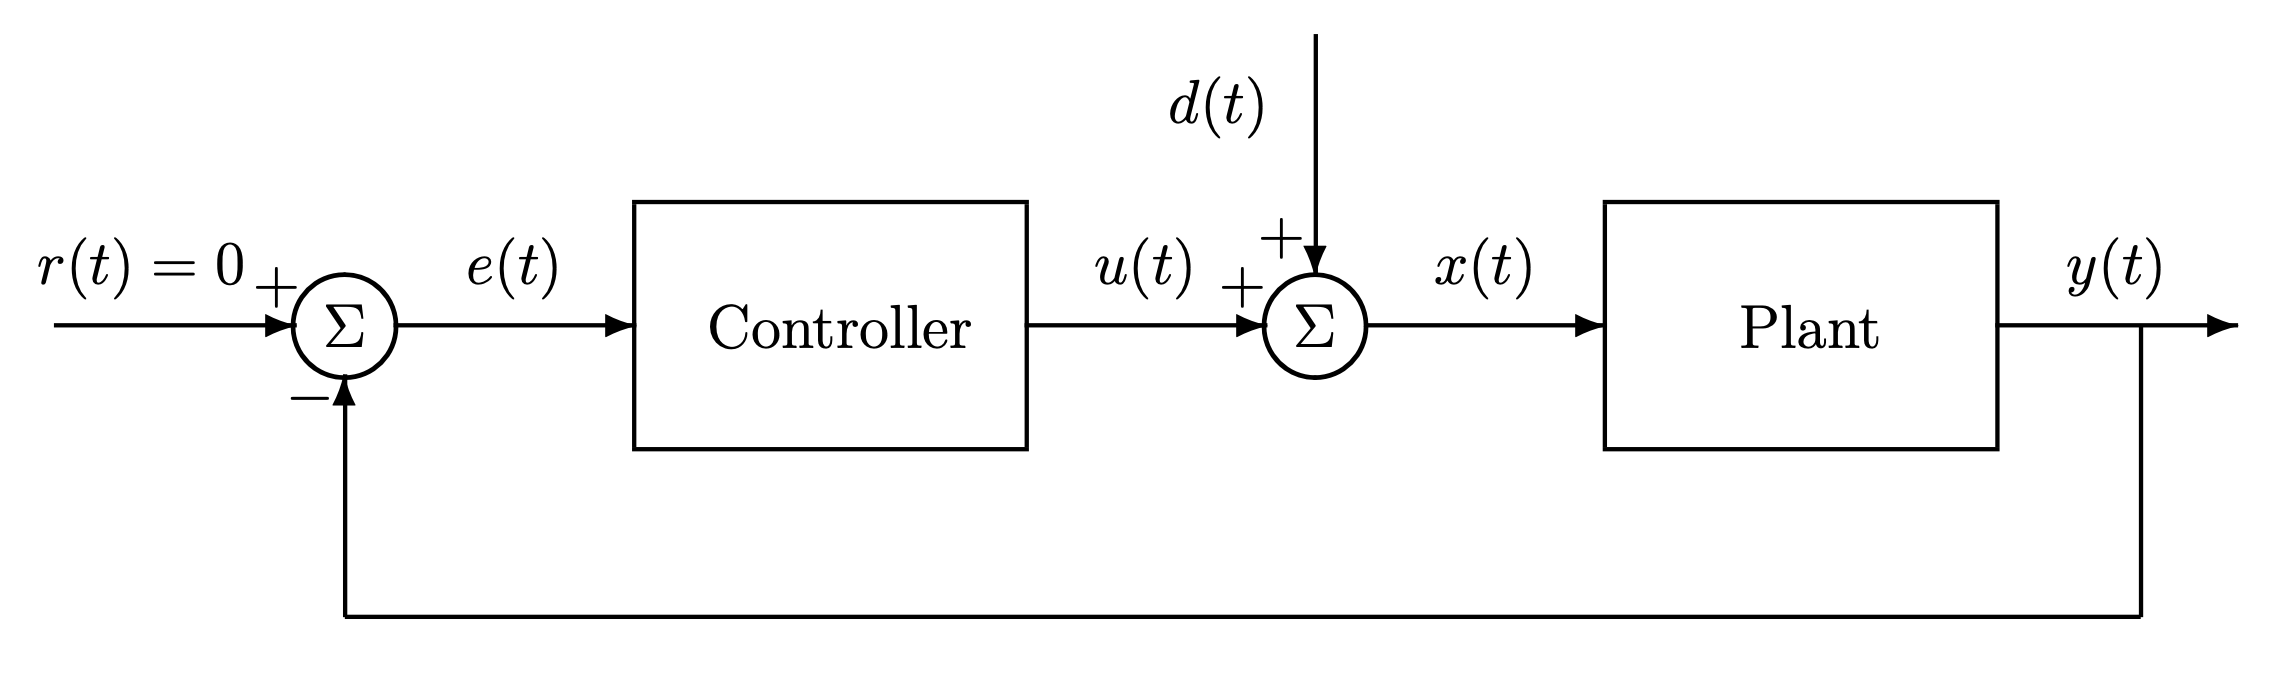
\includegraphics[width=0.5\textwidth]{images/block_diagram.png}
    \caption{Block diagram of the control system.}
    \label{fig:figure0}
\end{figure}

The controller can be manually controlled by a pilot, or automatically controlled by an autopilot.
The objective of both controllers is to minimise the error signal, $e(t)$, which is the difference between the desired output, $r(t)$ and the actual output, $y(t)$.
For this lab, the desired output, or the pitch of the aircraft is taken to be zero, and so the error signal is equal to the output signal.
There are however, disturbances to the system, $d(t)$, which cause the output to deviate from the desired output.
The signals $u(t)$ and $x(t)$ are the control output and the input to the plant respectively.

\section{Manual Aircraft Control}

\subsection{Simplified Aircraft Model}

A simplified model for aircraft dynamics is given by the following equation:

\[
 \ddot{y}(t) + M\dot{y}(t) = Nx(t)
\]

Where the coefficient $M$ represents the aerodynamic damping and coefficient $N$ represents aerodynamic effectiveness of elevators.
The transfer function of this system is given by:

\begin{equation}
    G_1(s) = \frac{N}{s(s + M)}
\end{equation}

\subsection{Manual control response to impulse disturbance}

The model for manual control by a pilot is taken as a pure time delay $D$ and a gain $k$ and so for an input response $x(t)$ the output is given as $kx(t-D)$. This has a transfer function in the laplace domain as seen below.

\begin{equation}
    K(s) = ke^{-sD}
\end{equation}

\begin{figure}[H]
    \centering
    \begin{subfigure}[t]{0.48\textwidth}
        \centering
        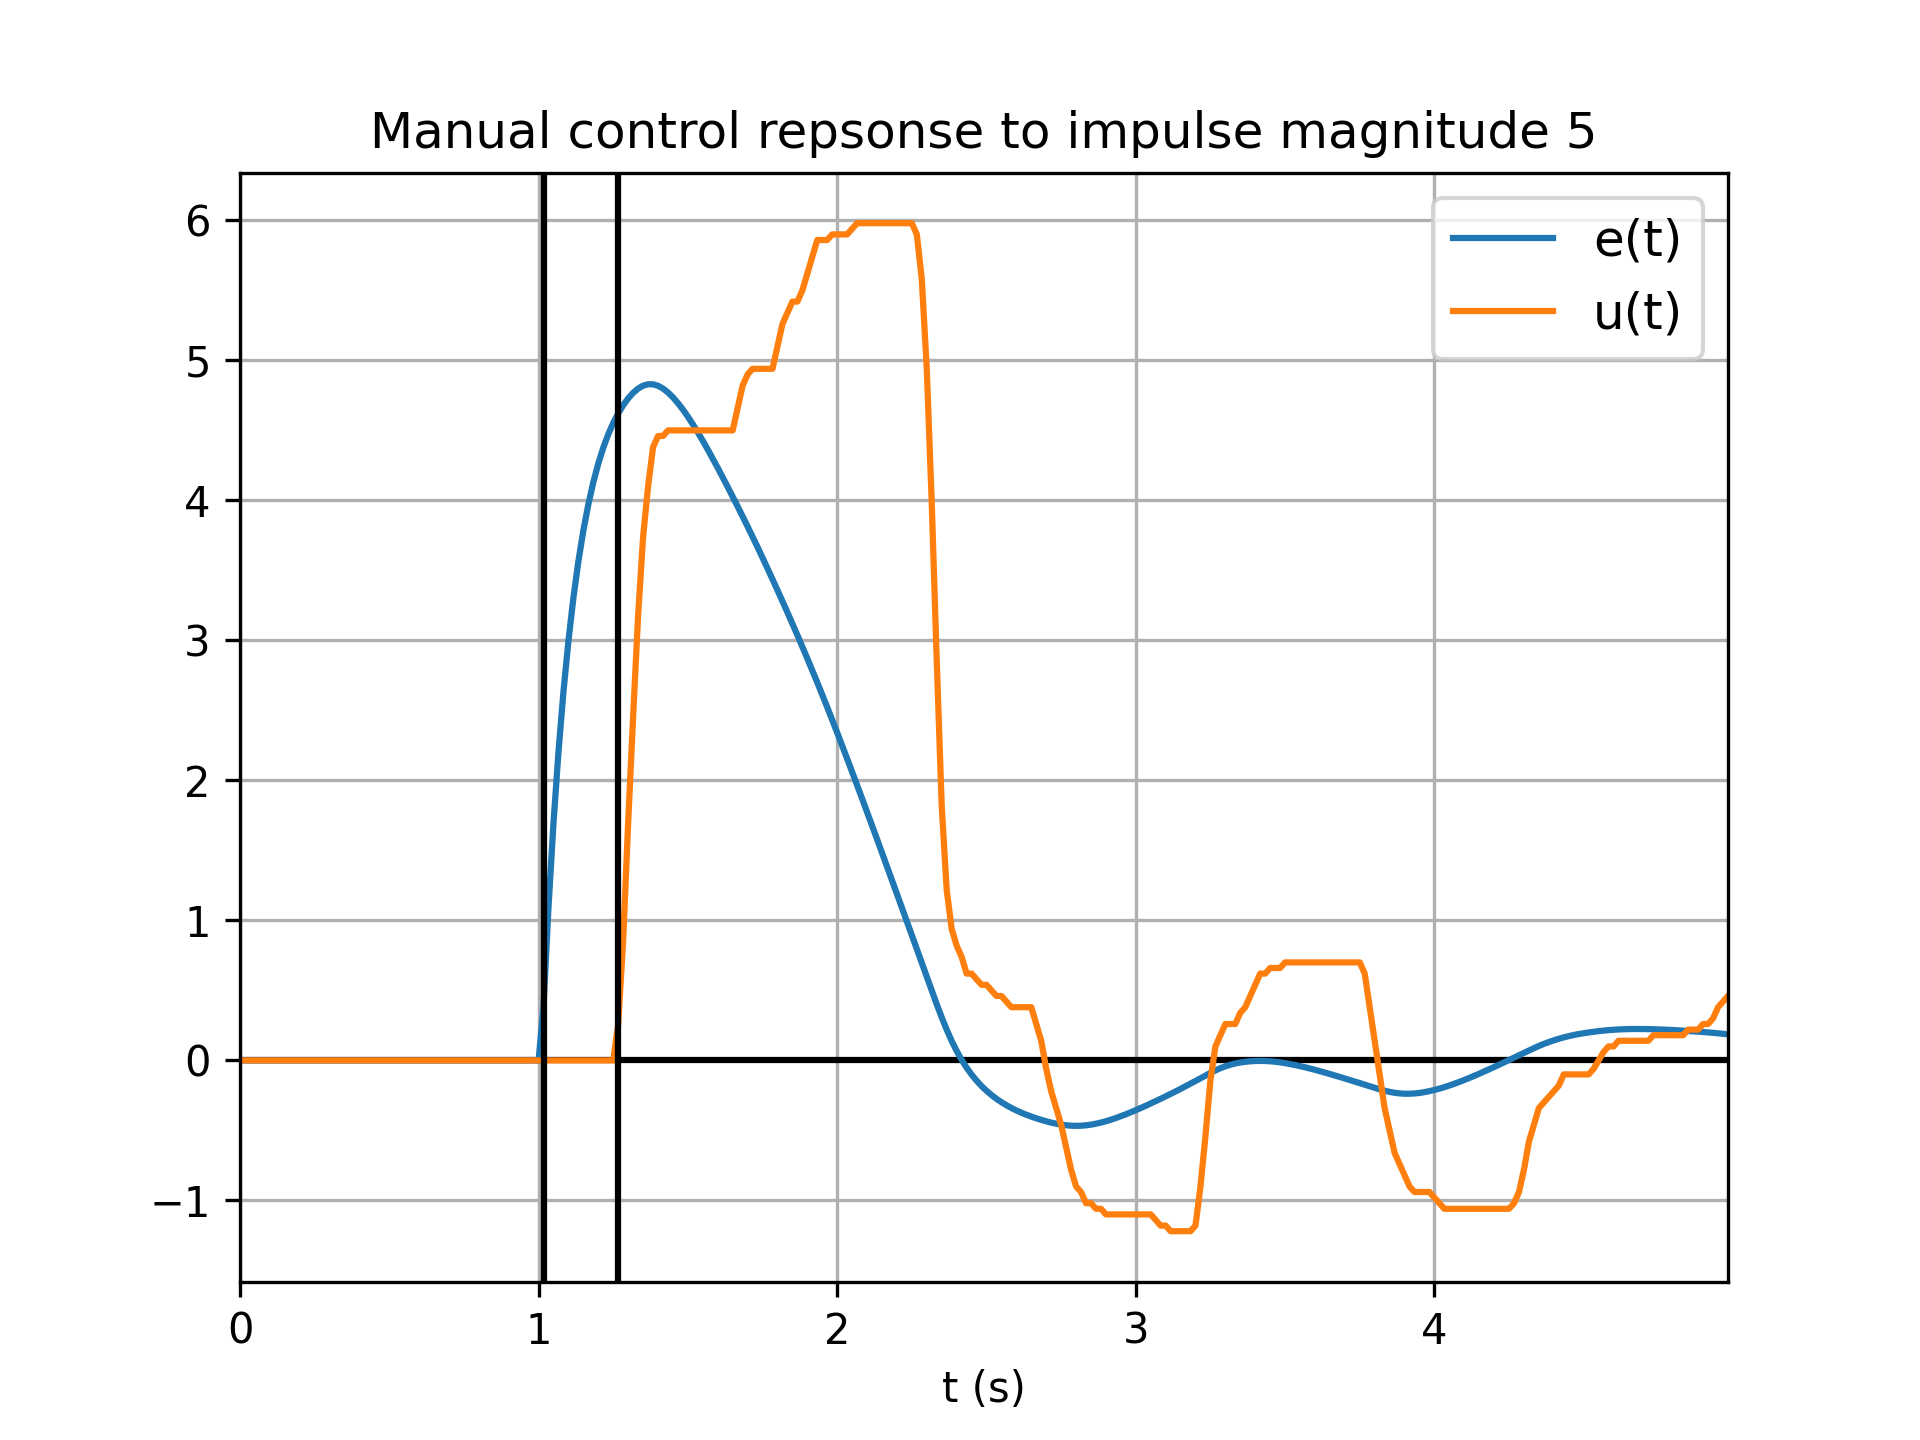
\includegraphics[width=1\textwidth]{figures/FIGURE_1.png}
        \caption{Manual control response graph to impulse disturbance.}
        \label{fig:figure1}
    \end{subfigure}
    ~
    \begin{subfigure}[t]{0.48\textwidth}
        \centering
        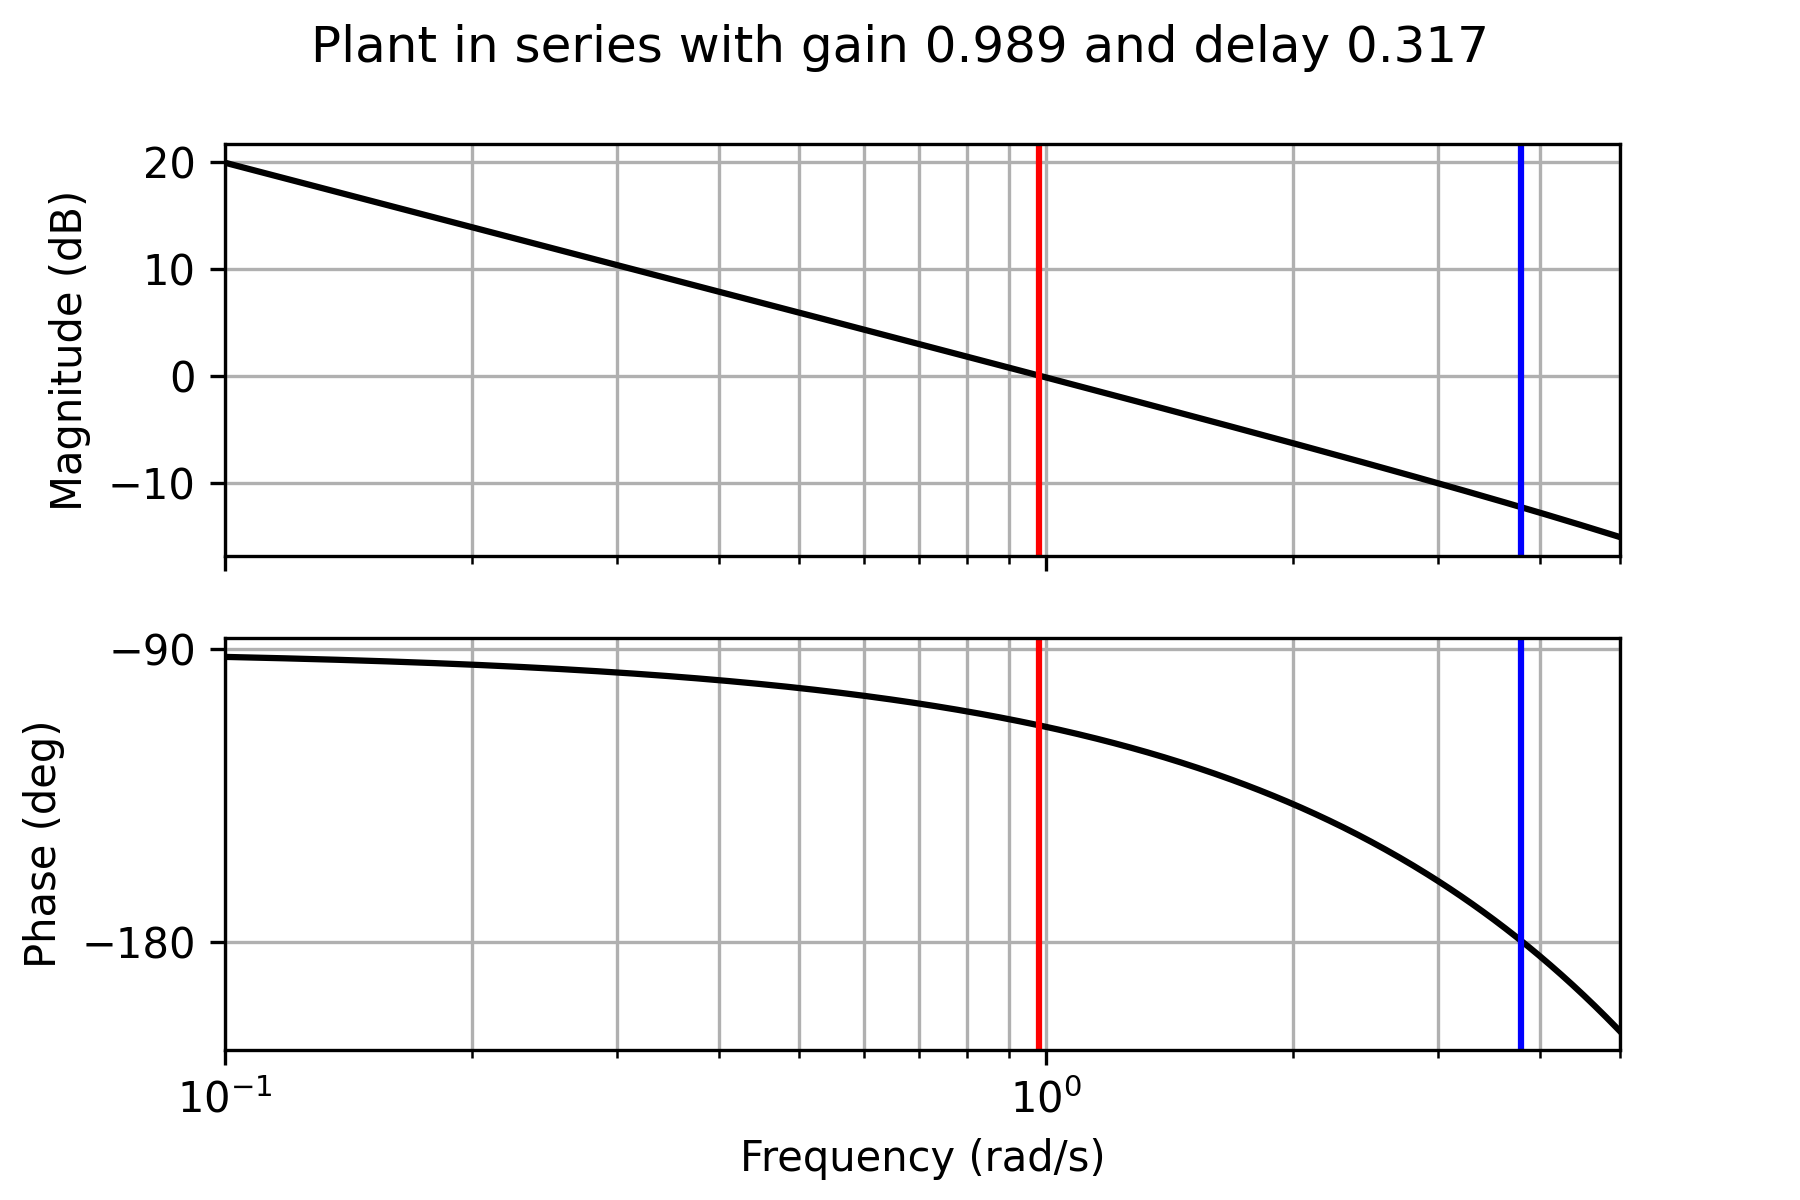
\includegraphics[width=1\textwidth]{figures/FIGURE_2.png}
        \caption{Bode plot of open loop modelled manual control.}
        \label{fig:figure2}
    \end{subfigure}
    \caption{Manual control response}
\end{figure}

From Figure \ref{fig:figure1}, the gain is determined by the ratio of control siganl to error signal peaks input and the time delay is determined by the time difference between the rise of the input and output.
These were found to be $1.238$ and $0.250$ s respectively.

From Figure \ref{fig:figure2}, the gain margin is found using the gain on at the blue line at at -180 degrees phase. This was found to be $4.03$.
The phase margin is found using the phase difference with -180 on the red line where the gain is 0dB. This was found to be $65.4$ degrees. Both of these points correspond to where the nyquist plot encircles the $-1$ point.

If the gain of $1.238$ were to remain unchanged, from the frequency of $\omega = 1.228$ rad/s at the phase margin of $65.4$ degrees the additional time delay before unstability be found to be $0.929$ s.

\begin{figure}[H]
    \centering
    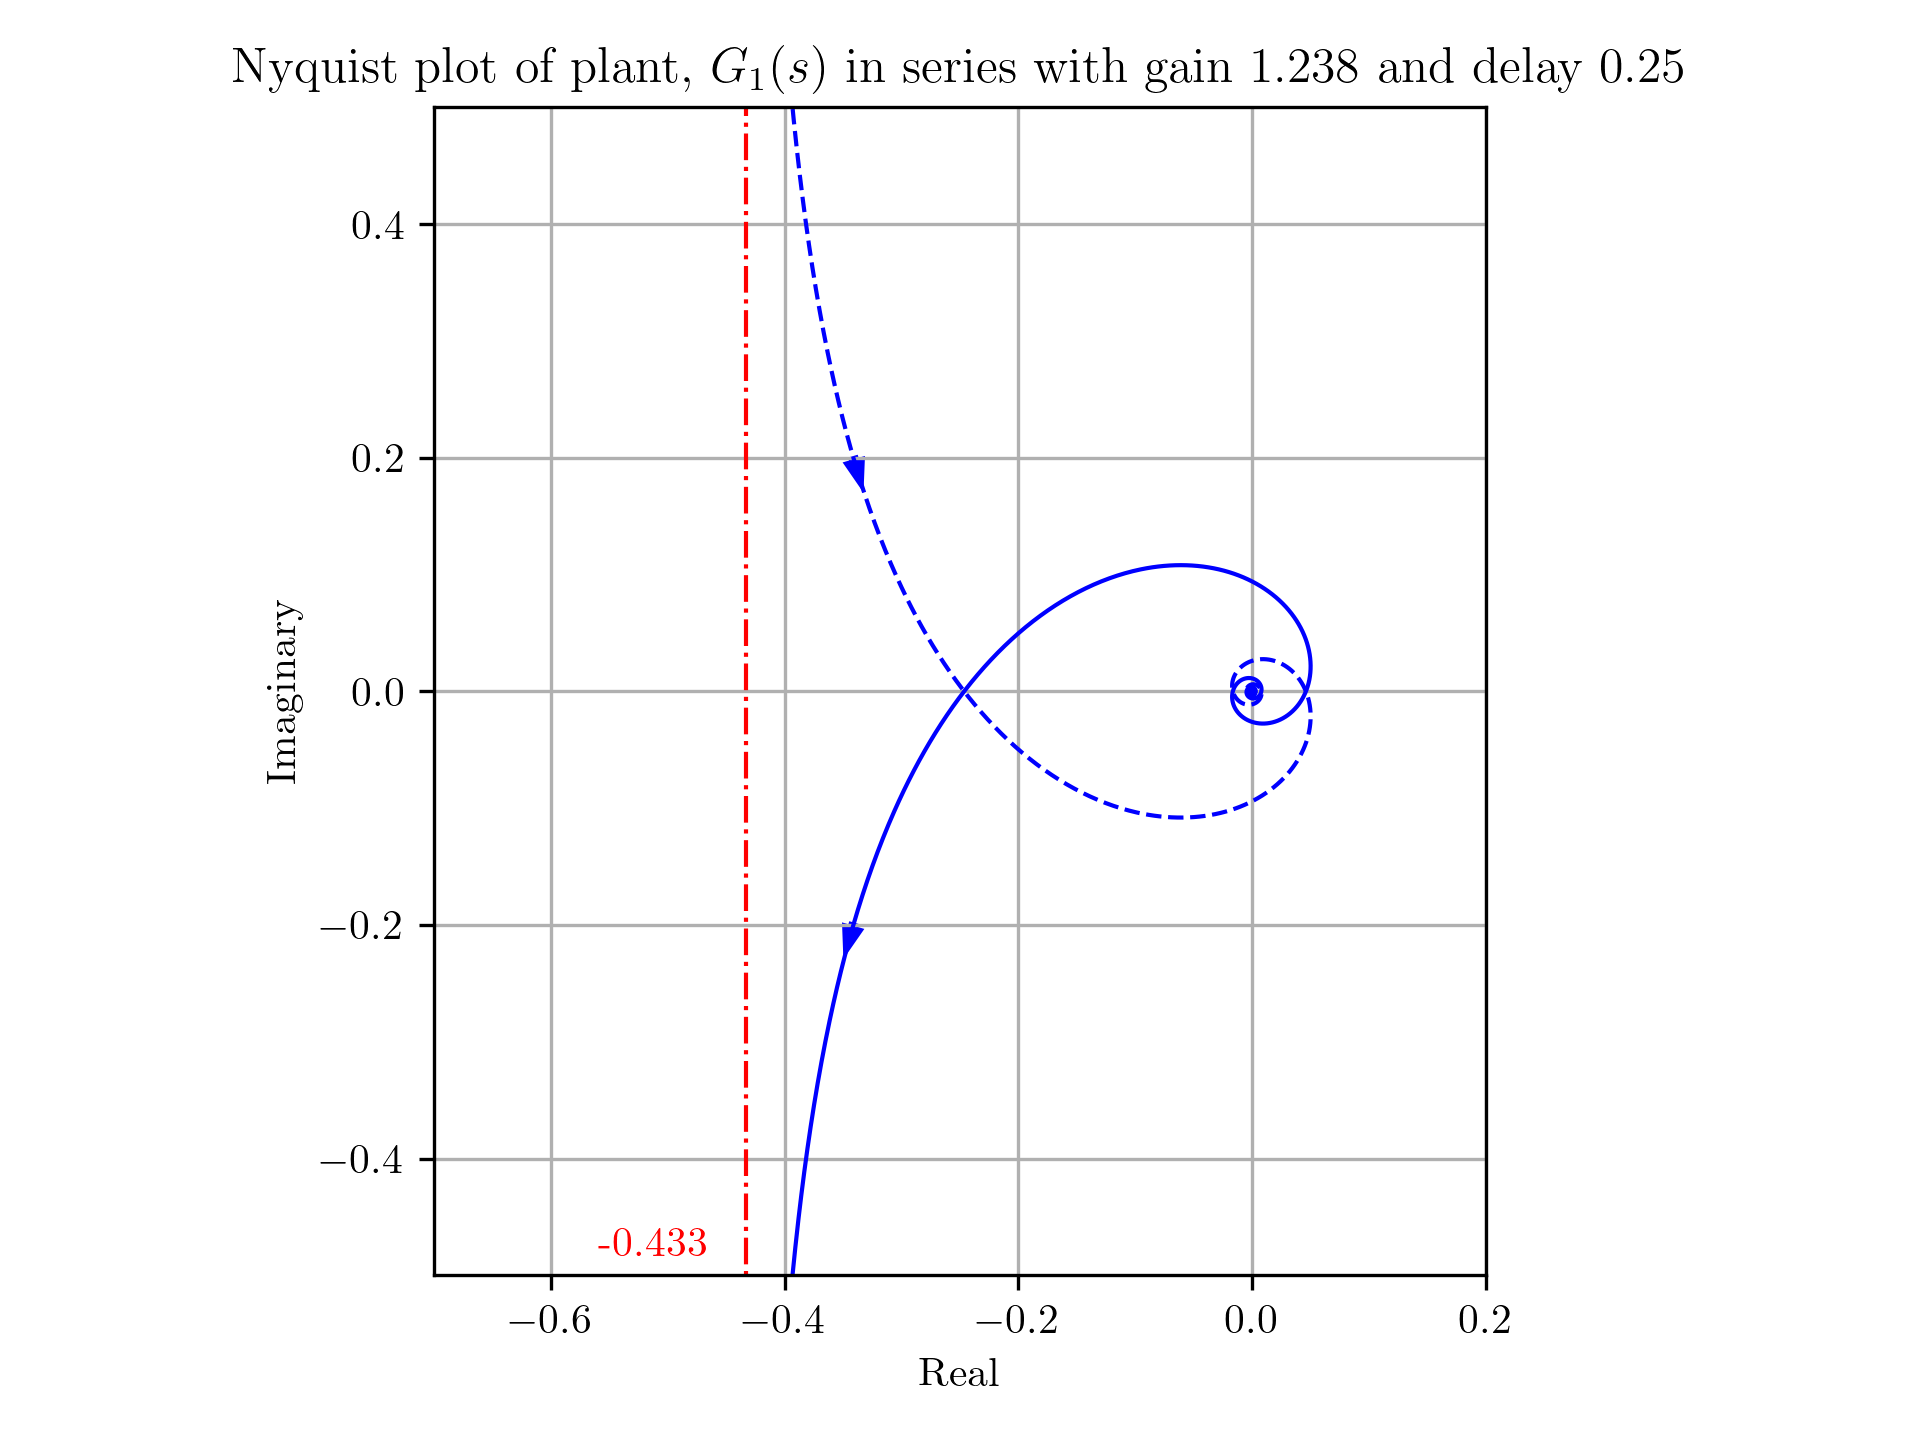
\includegraphics[width=0.8\textwidth]{figures/nyquist1.png}
    \caption{Nyquist plot for open loop manual control model, $K(s)G(s)$.}
    \label{fig:nyquist1}
\end{figure}
% could do additional nyquist plots at cases of gain and phase margins.

\subsection{Manual response to step input disturbance}

\begin{figure}[H]
    \centering
    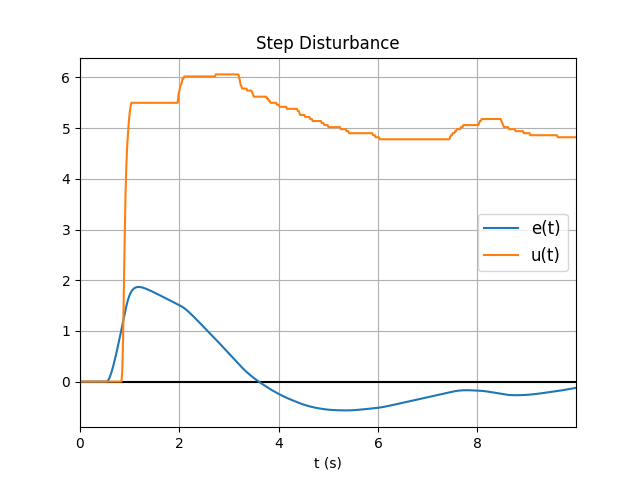
\includegraphics[width=0.8\textwidth]{figures/FIGURE_3.png}
    \caption{Manual control response to step disturbance.}
    \label{fig:figure3}
\end{figure}

In Figure \ref{fig:figure3} the manual control to the step response can be seen. It can be seen that integral action is used here, as to minimise the error signal $e(t)$ to 0, the input signal $u(t)$ must equal a constant final value, which can only be achieved by an intergator.
The original model for the controller without the intregral term would have a large error.

The control input is still delayed a time, $D$, to the error signal, but now with an intergator term, so we would expect the new controller to take the form of a proportional integrator, (PI), controller:

\begin{equation}
    K(s) = e^{-sD}\left( k + \frac{1}{sT_i}\right)
\end{equation}

\section{Pilot Induced Oscillation}

Considering an aircraft of poorly designed control system with the transfer function.

\begin{equation}
    G_1(s) = \frac{c}{(Ts+1)^3}
\end{equation}

Where parameters are chosen as: $T=4D/\pi$ and $c=\sqrt{8}/k$
An impulse response of $5kD$ is shown below in Figure \ref{fig:figure4}.

\begin{figure}[H]
    \centering
    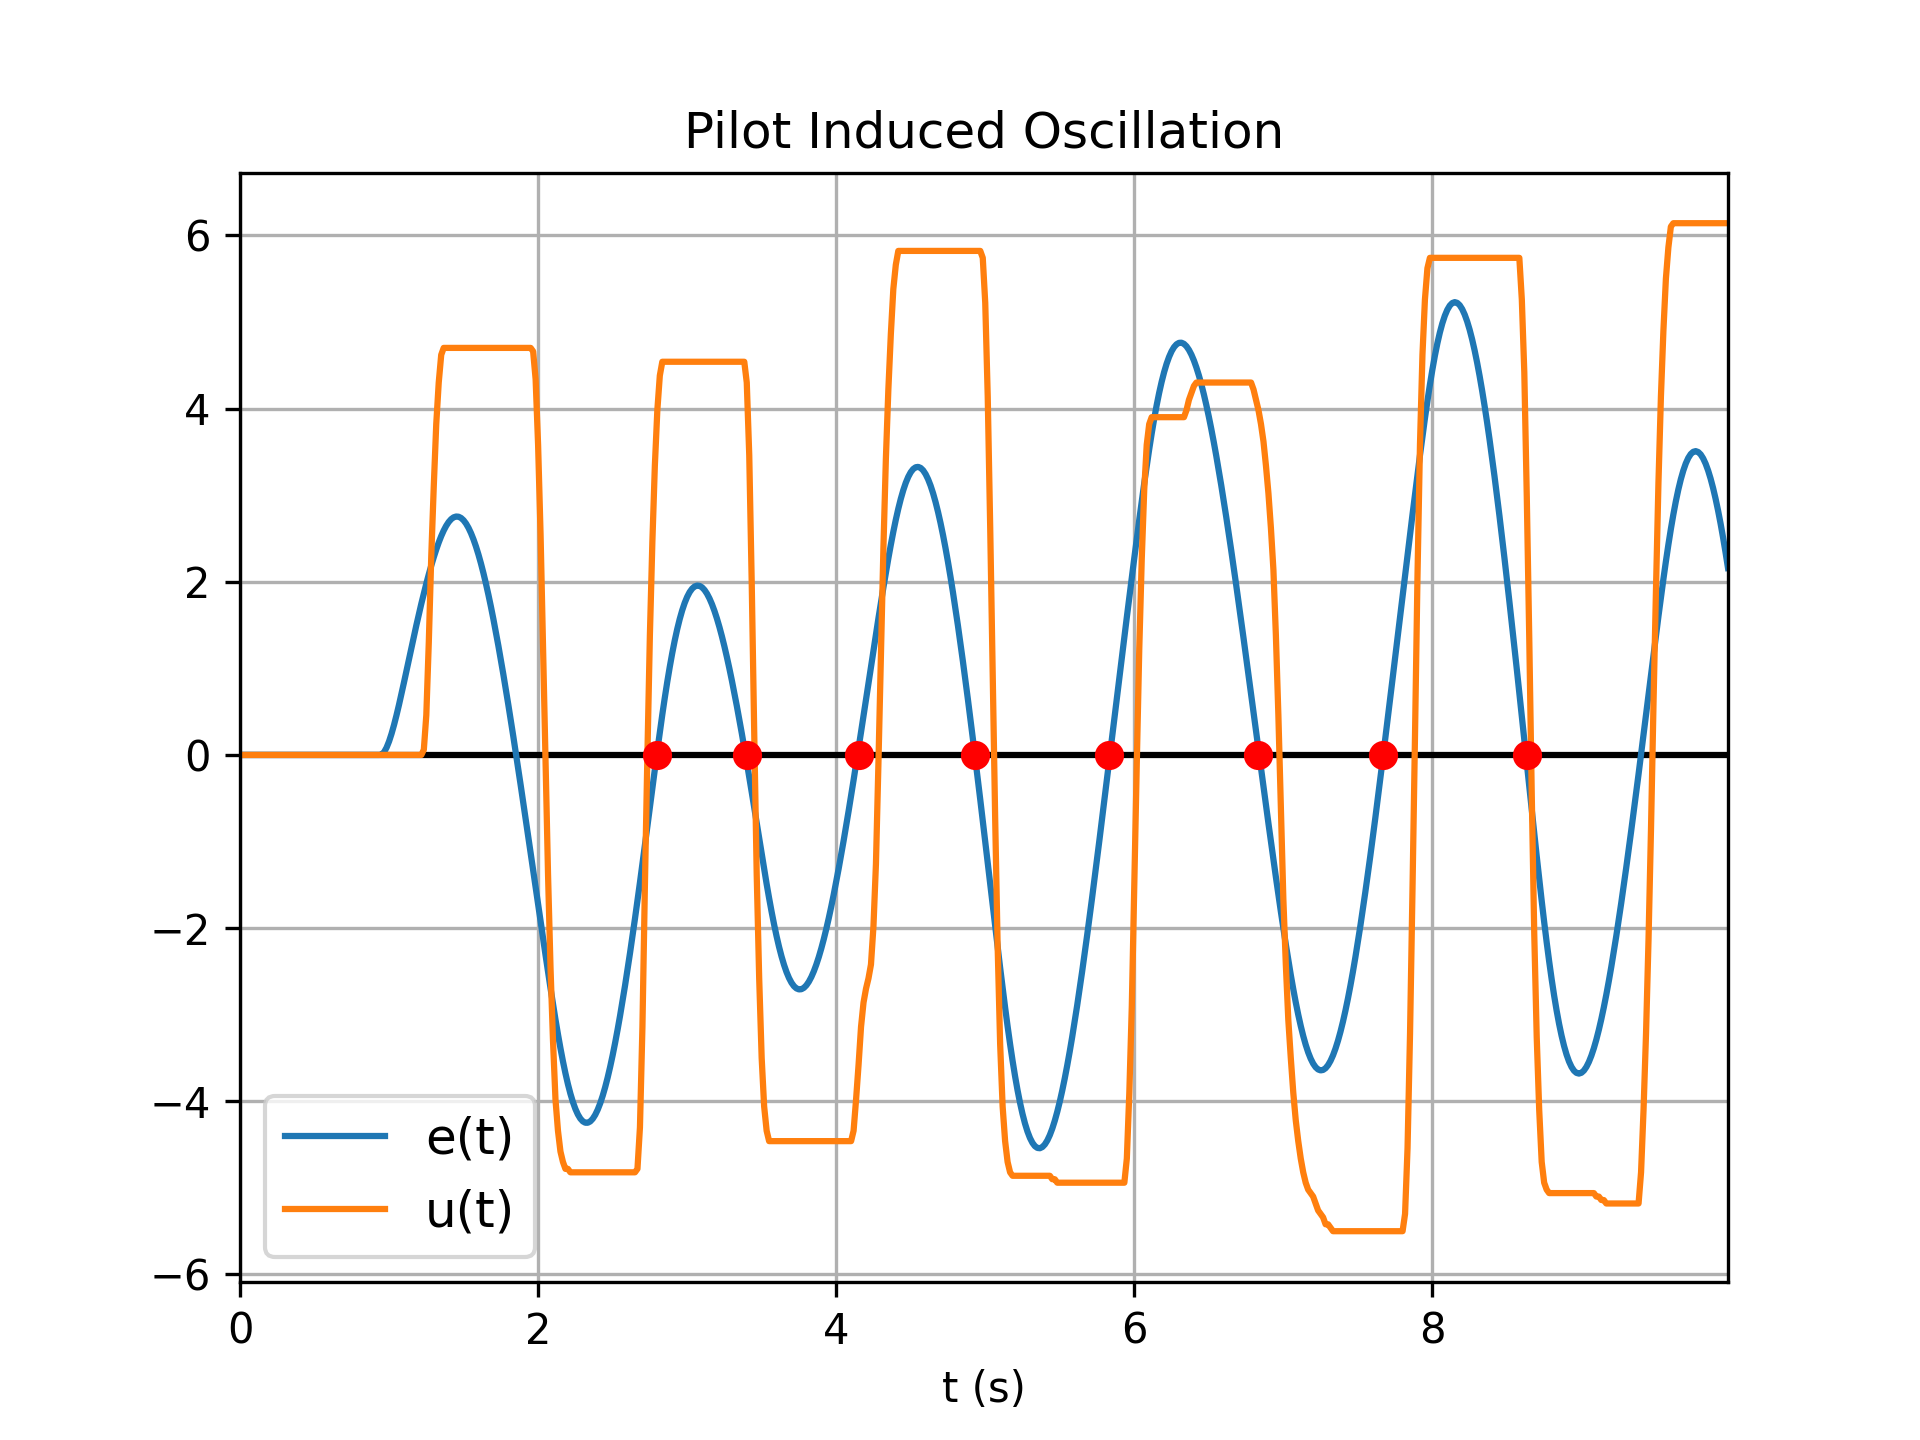
\includegraphics[width=0.8\textwidth]{figures/FIGURE_4.png}
    \caption{Manual control response to impulse disturbance of weight $5kD$.}
    \label{fig:figure4}
\end{figure}


This shows a highly oscillatory response triggered by the impulse disturbance.
The average period of which is $1.654$ s, as calculated from where the error signal intersects the x axis shown by the red points.

The response for the modelled pilot controller, with same gain and delay as before is shown below in Figure \ref{fig:figure5}.

\begin{figure}[H]
    \centering
    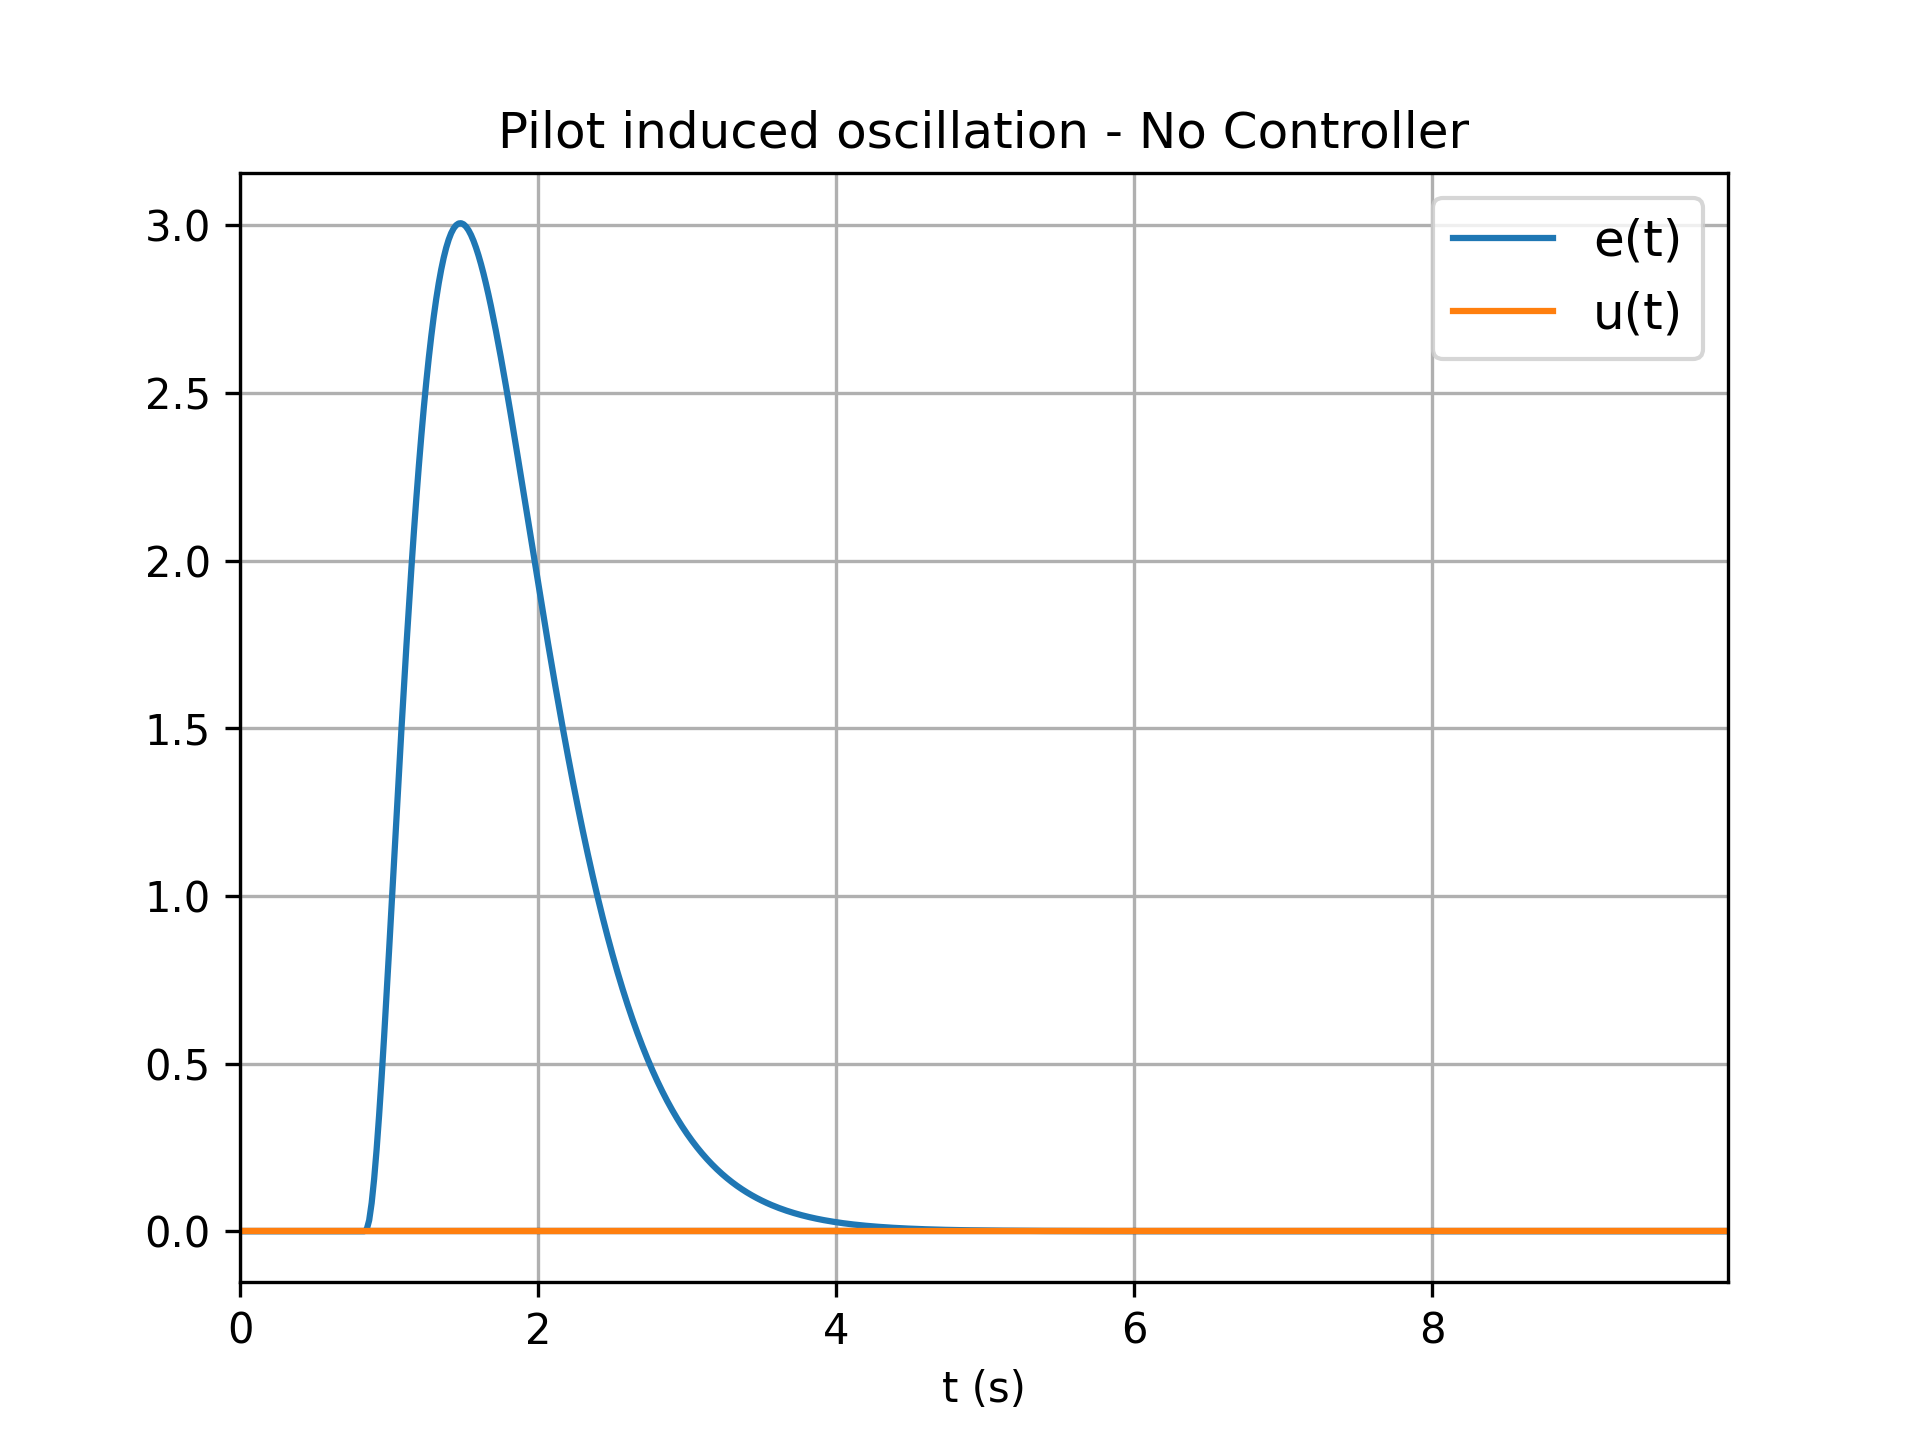
\includegraphics[width=0.8\textwidth]{figures/FIGURE_5.png}
    \caption{No controller response to impulse disturbance of weight $5kD$.}
    \label{fig:figure5}
\end{figure}

In Figure \ref{fig:figure5} without a controller, shows no oscillatory response, to the same impulse disturbance.

\begin{figure}[H]
    \centering
    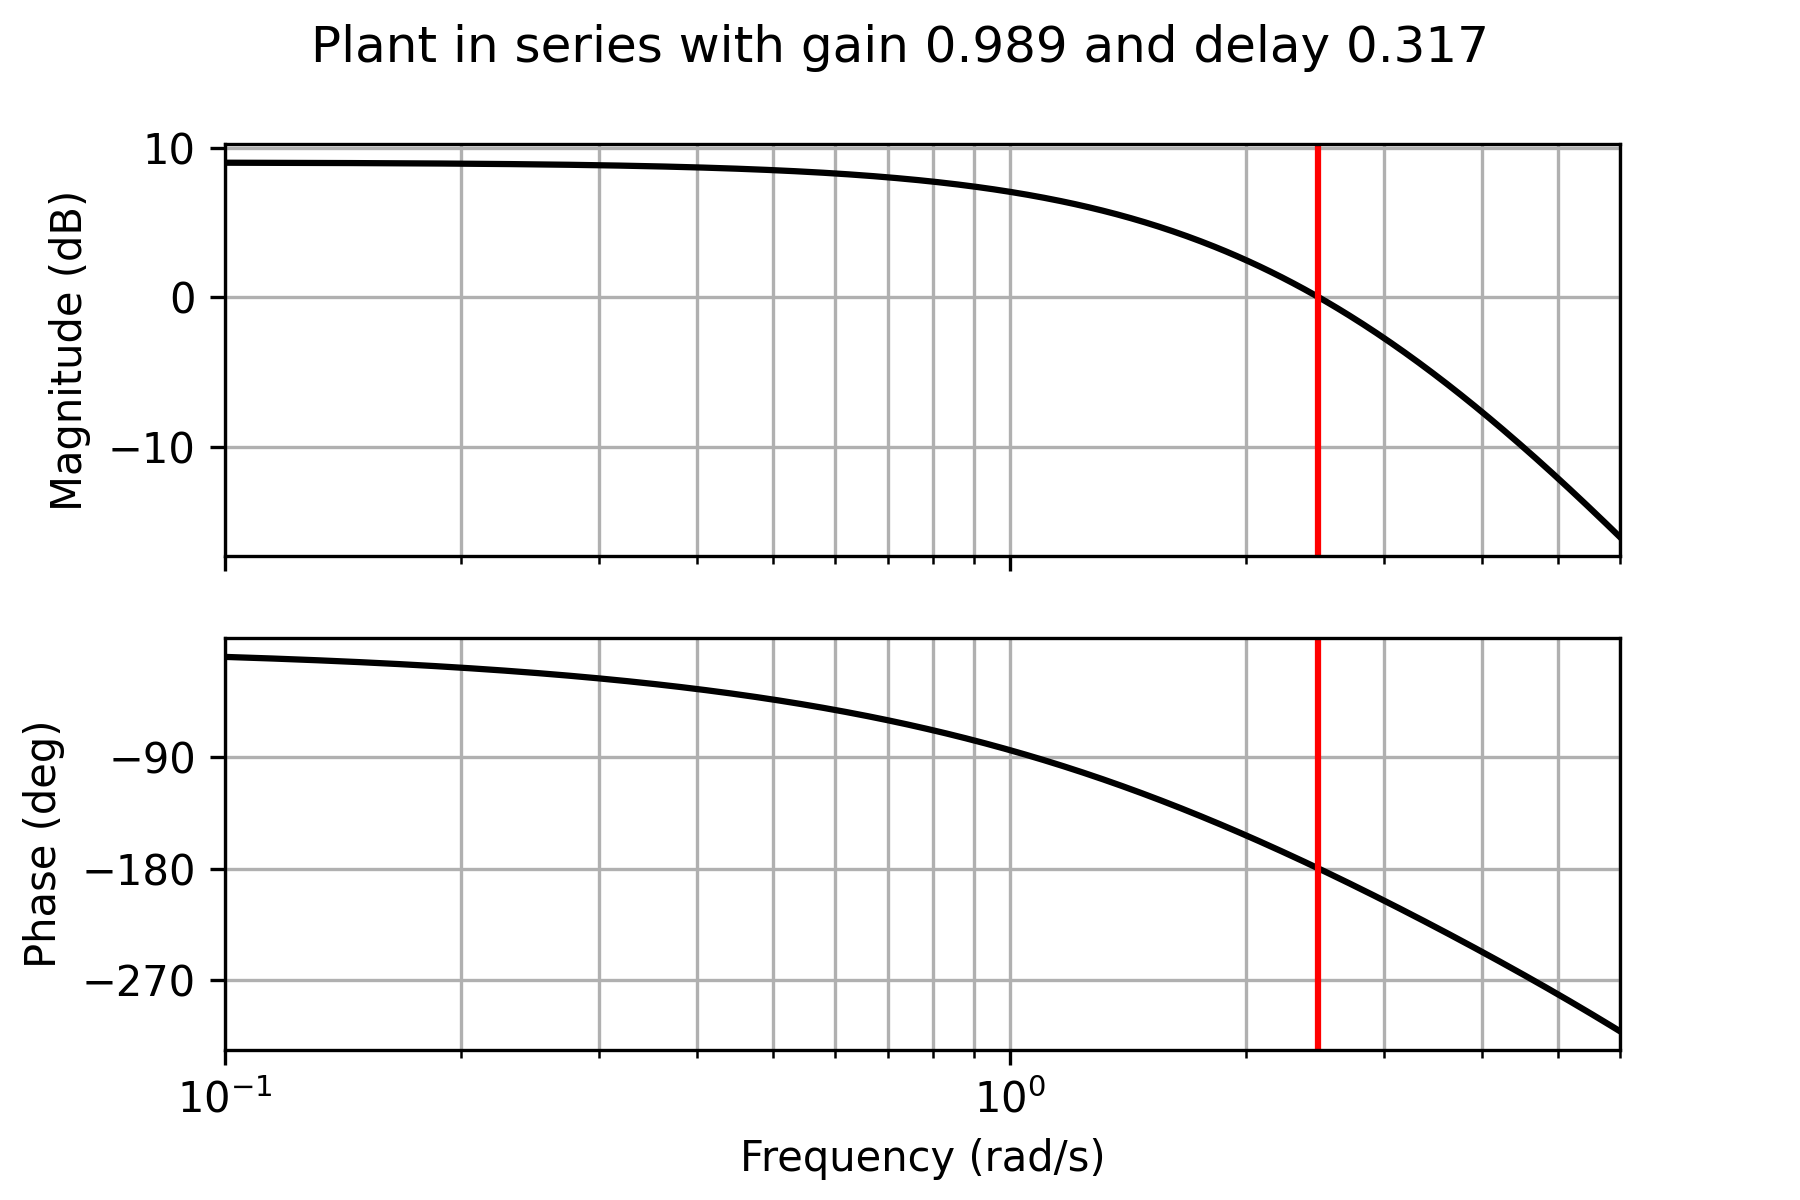
\includegraphics[width=0.8\textwidth]{figures/FIGURE_6.png}
    \caption{Bode plot of, $K(s)G(s)$.}
    \label{fig:figure6}
\end{figure}

Figure \ref{fig:figure6} shows the bode plot of the plant, $G_2(j\omega)$ in series with the model pilot controller.
The gain and phase margins are found the same way as \ref{fig:figure2} and are found to be, 0.997 and 0.212 degrees respectively.
This is on the edge of stability, and so for a large, or slow response from the pilot, the system can become unstable.

At this point of unstability, the frequency is found to be $\omega = 2.473$ rad/s, which corresponds to a theortical period of $2.540$ s.
This period of oscillation, is much larger than the period of oscillation of the real manual controller, which was $1.672$ s.
The blue line on the bode plot in \ref{fig:figure6} shows the measured frequency of oscillation. 
This corresponds to a smaller controller delay, suggesting that the pilot is responding much faster than the modelled pilot, perhaps predicting the oscillatory motion, in an attempt to stabalise.

A control system designer must ensure sufficient gain and phase margins to ensure stability of the system for a range of pilot responses.
This could be done by introducing a phase lead compensator to the system, which can increase both the gain and phase margins of the system, but may have the undesired effect of decreasing low frequency gain.

\newpage

\section{Sinusoidal Disturbances}

For this section, the control system of a F4E fighter jet is analysed during sinusoidal distrubances.
The fighter jet has various operating points, for which the dynamics of the system are linearised about these operating points, which are given by the transfer functions in table \ref{tab:1} below.

\renewcommand{\arraystretch}{2}
\begin{center}
    \captionof{table}{F4E fighter jet operating points}
    \begin{tabular}{|c|c|c|c|}
    \hline 
    Point & Altitude  &  Mach Number & Transfer Function\\
    & (ft.) & & \\
    \hline 
    1 & 5000 & 0.5 & $\frac{185.3521 s + 163.8444}{1.0 s^{4} + 15.8408 s^{3} + 22.0034 s^{2} - 52.7495 s}$ \\
    2 & 5000 & 0.85 & $\frac{507.7712 s + 789.0659}{1.0 s^{4} + 17.12 s^{3} + 34.93 s^{2} - 122.5005 s}$ \\
    3 & 35000 & 0.9 & $\frac{158.3182 s + 101.8049}{1.0 s^{4} + 15.3257 s^{3} + 17.514 s^{2} - 14.6419 s}$ \\
    4 & 35000 & 1.5 & $\frac{304.2262 s + 251.4097}{1.0 s^{4} + 15.7412 s^{3} + 43.6008 s^{2} + 269.1355 s}$ \\
    \hline
    \end{tabular}
    \label{tab:1}
\end{center}

The first three operating points are unstable and are near impossible to control manually.
The fourth operating point is stable with a lightly damped mode and can be controlled manually.
An attempt to stabalise the aircraft, given a sinusoidal disturbance of $0.66$Hz can be seen in Figure \ref{fig:figure7}.

\begin{figure}[H]
    \centering
    \begin{subfigure}[t]{0.48\textwidth}
        \centering
        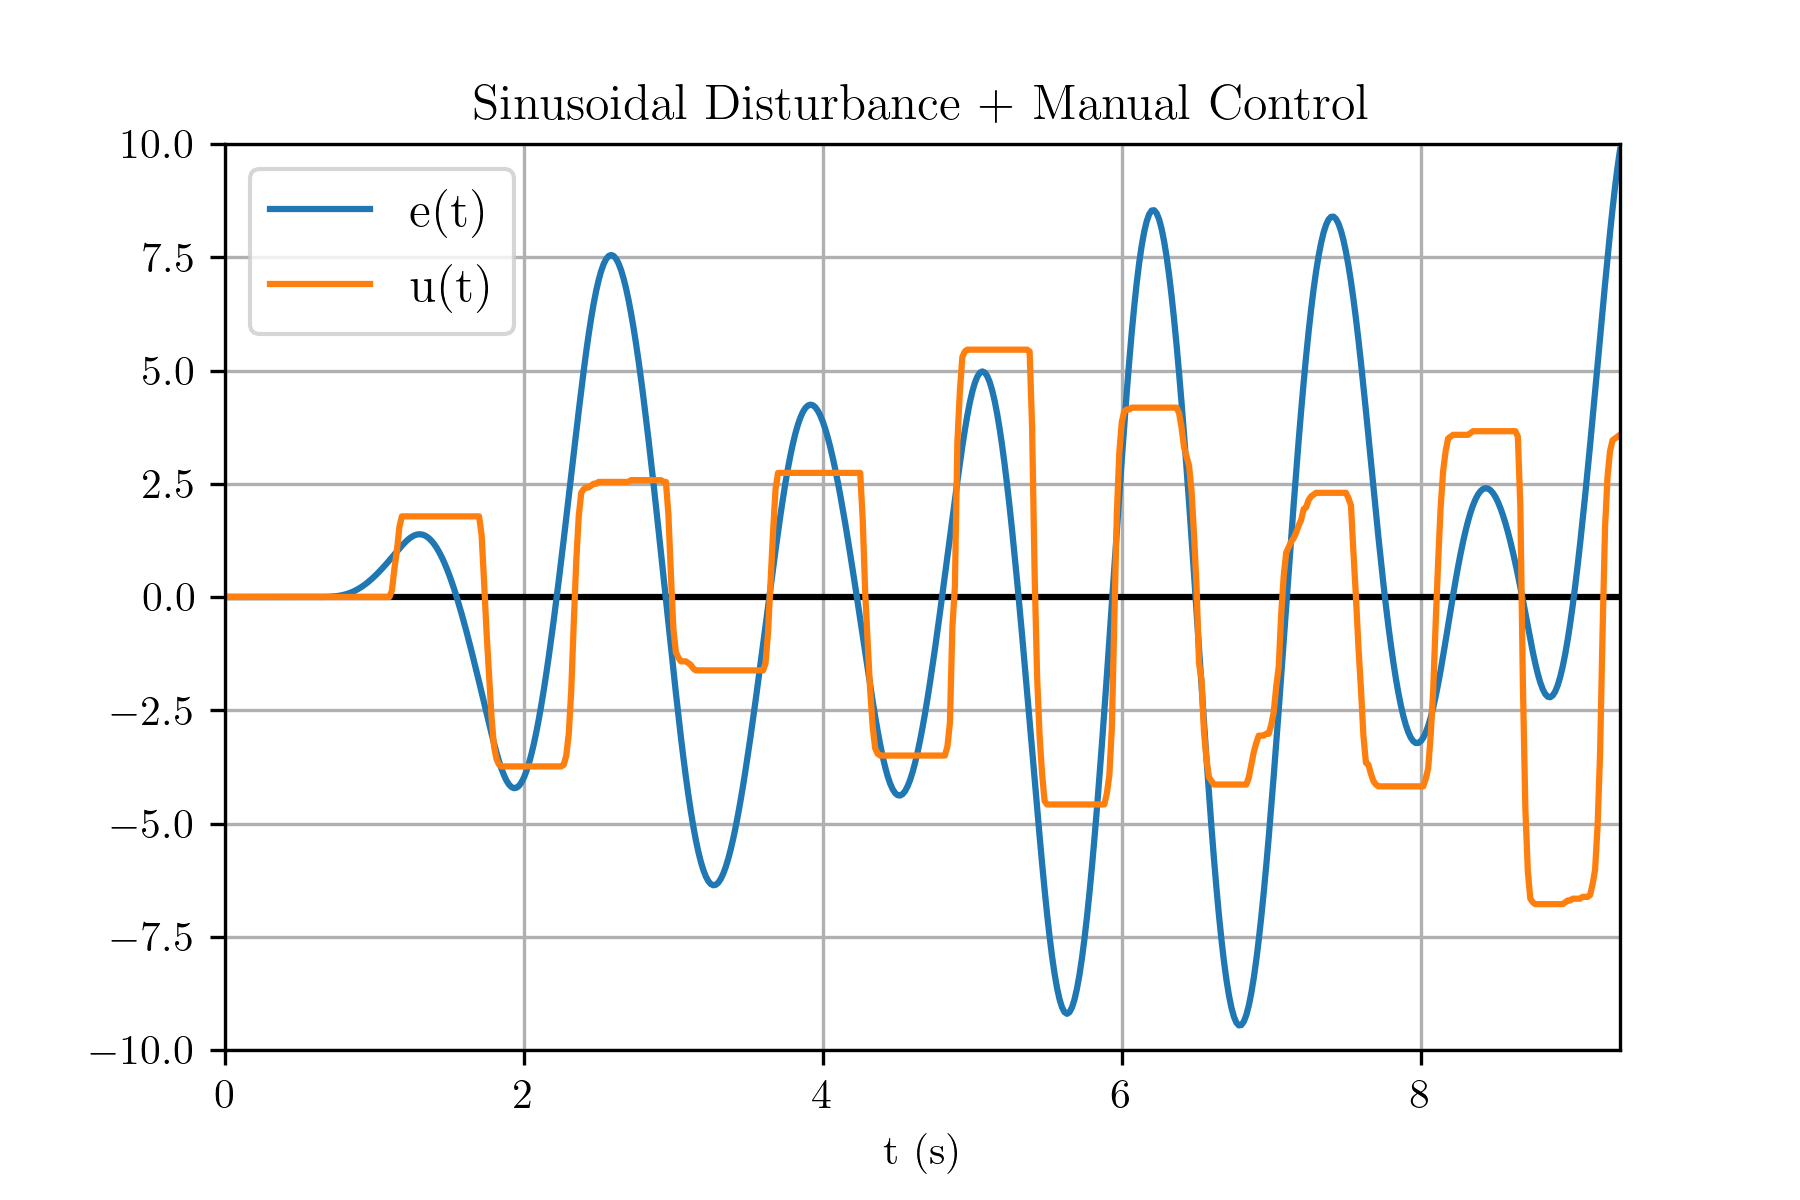
\includegraphics[width=1\textwidth]{figures/FIGURE_7.png}
        \caption{Manual control input response with $0.66$ Hz sinusoidal disturbance.}
        \label{fig:figure7}
    \end{subfigure}
    ~
    \begin{subfigure}[t]{0.48\textwidth}
        \centering
        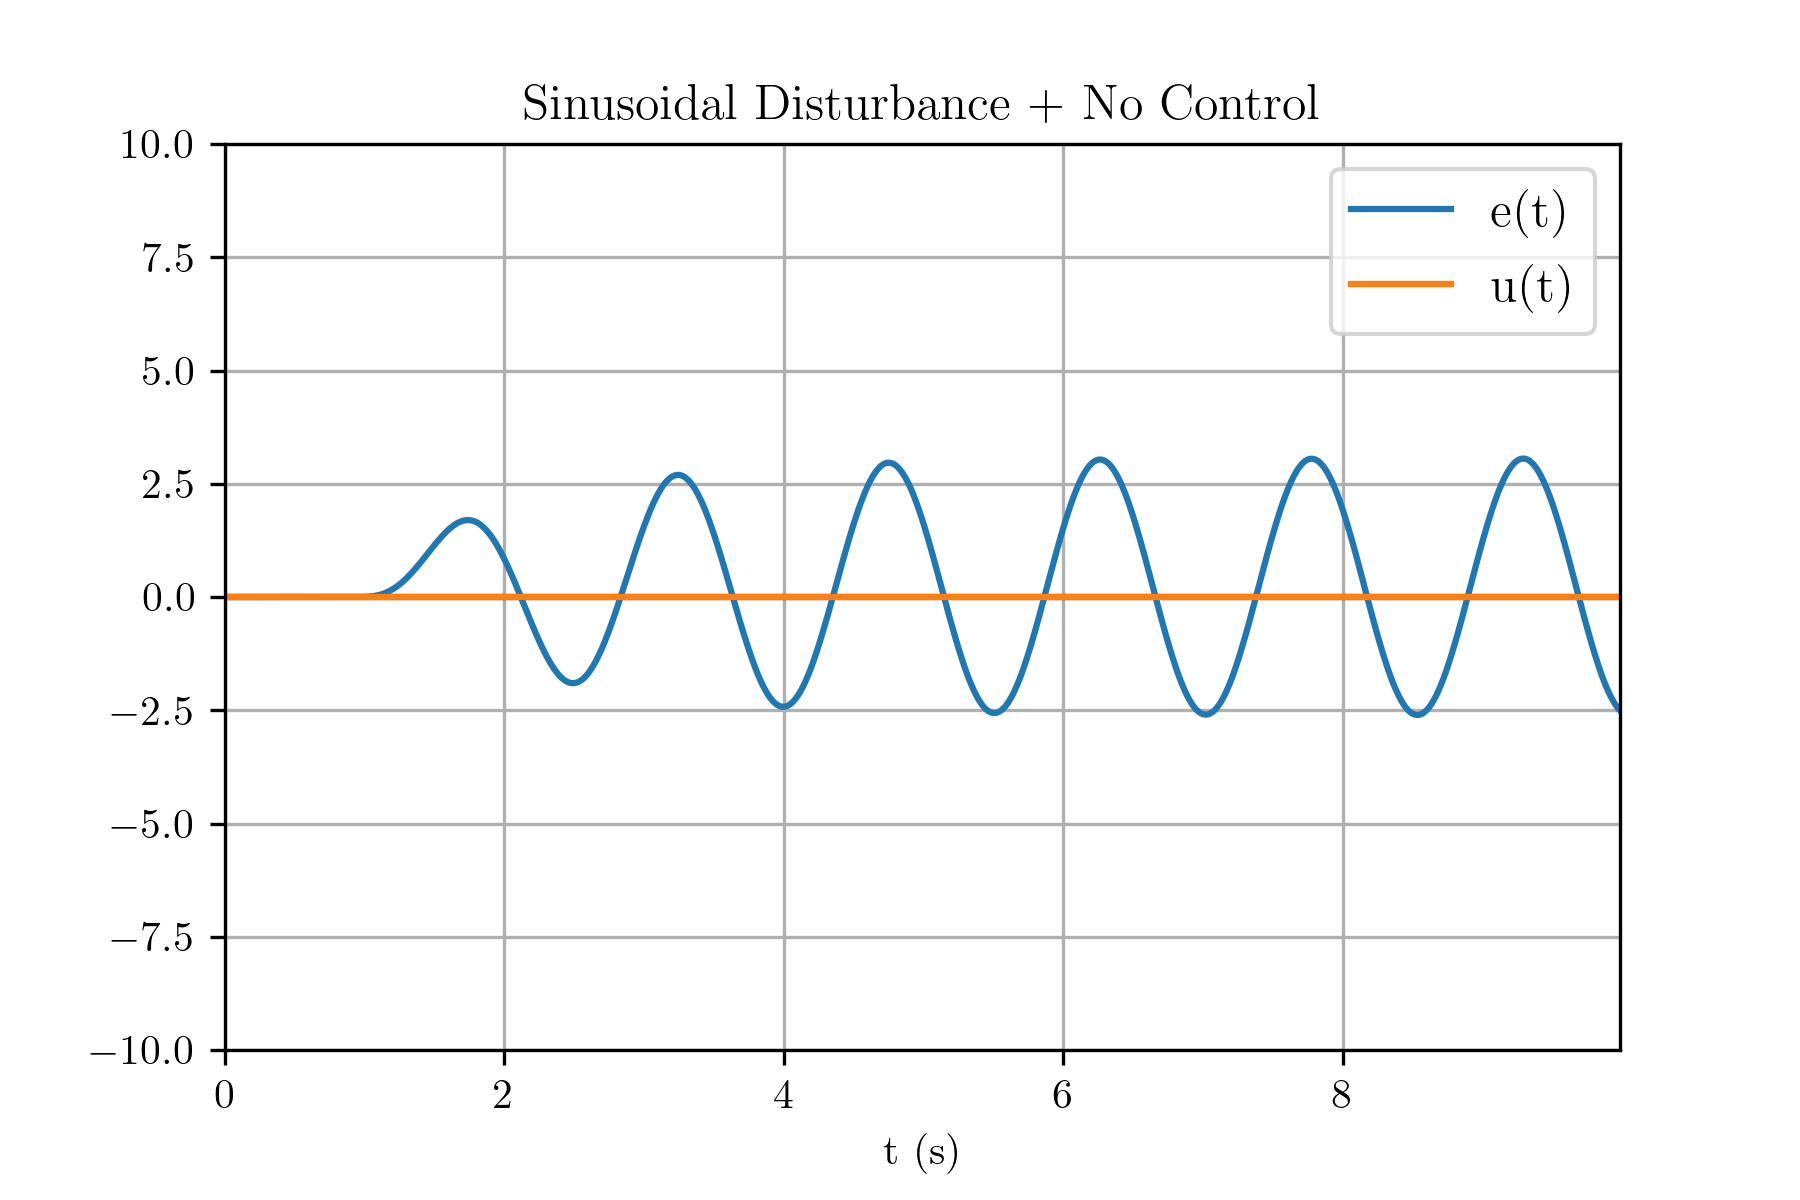
\includegraphics[width=1\textwidth]{figures/FIGURE_8.png}
        \caption{No control input response to $0.66$ Hz sinusoidal disturbance.}
        \label{fig:figure8}
    \end{subfigure}

    \begin{subfigure}[t]{0.48\textwidth}
        \centering
        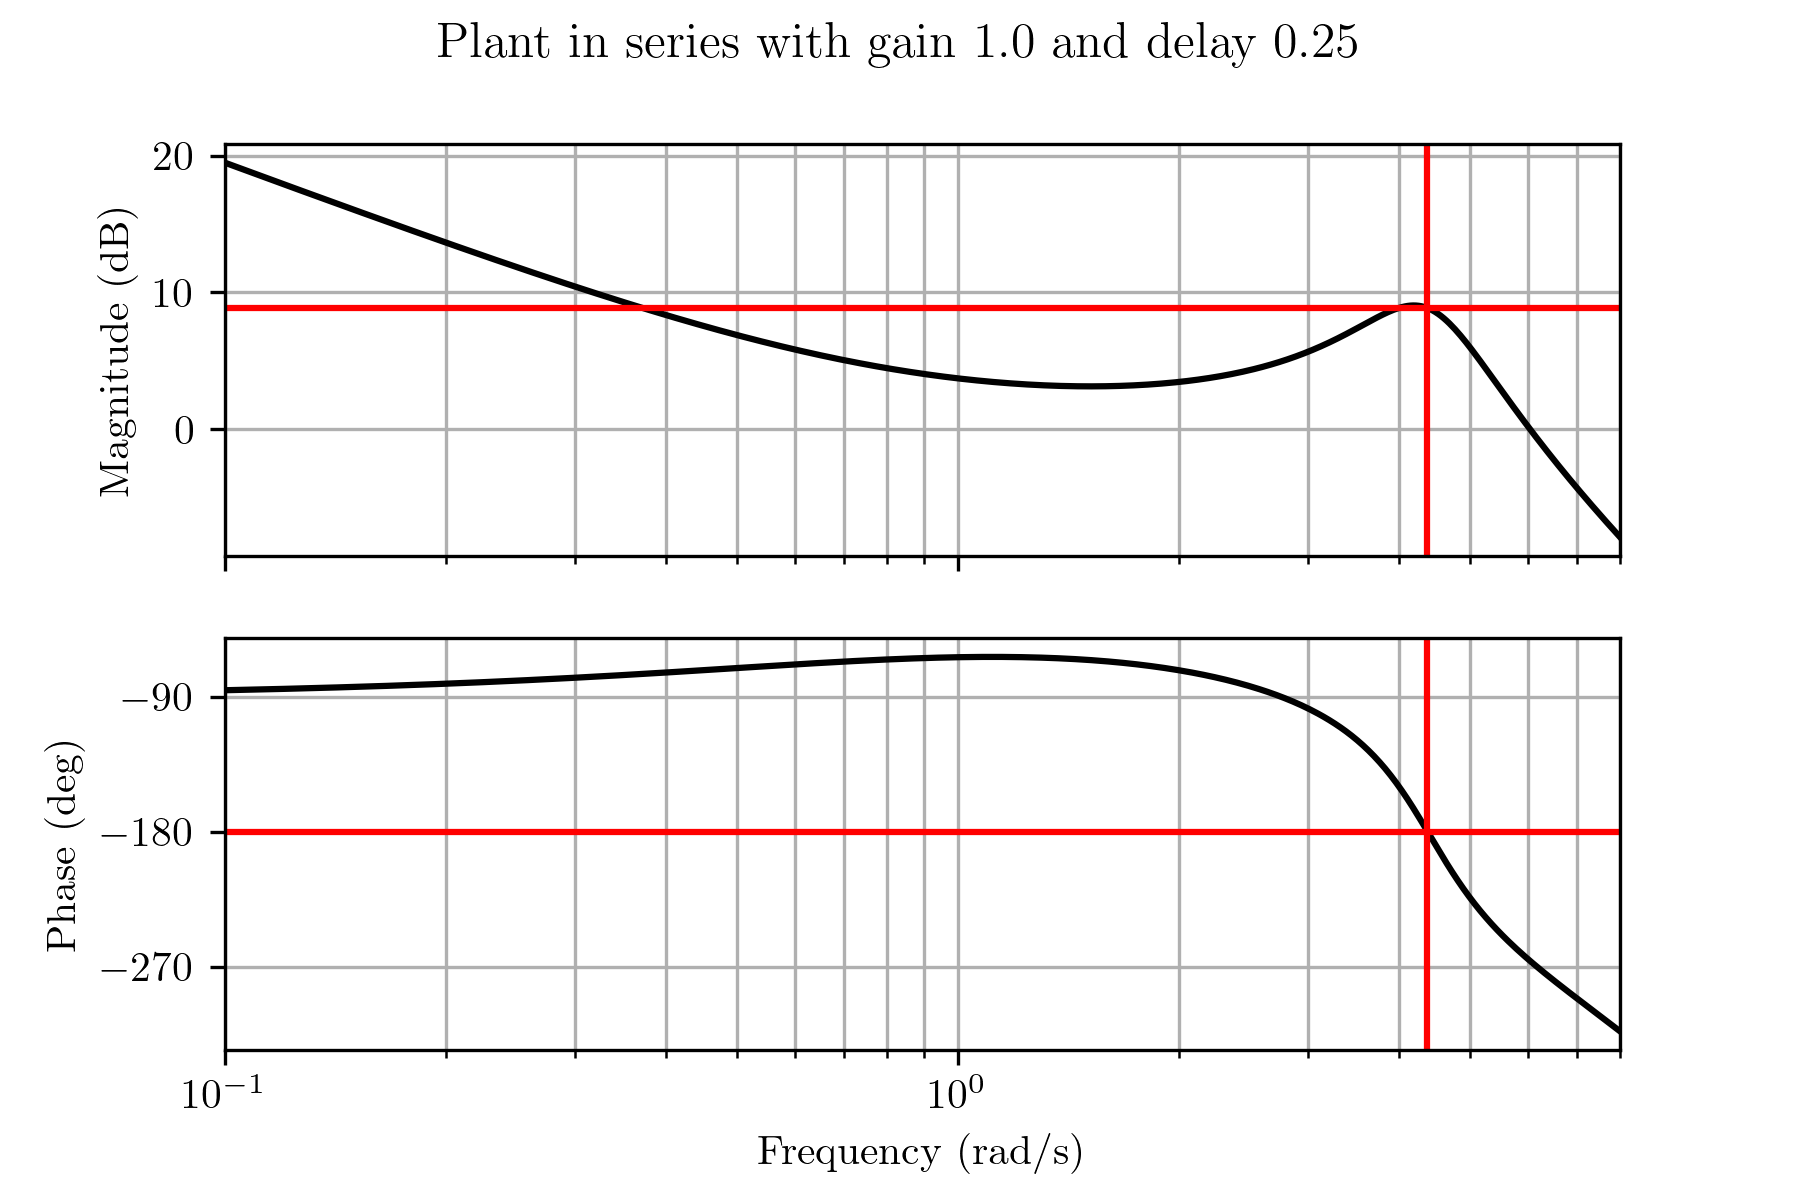
\includegraphics[width=1\textwidth]{figures/FIGURE_9.png}
        \caption{Bode plot for F4E fighter jet with controller of gain $1.0$ and time delay $0.250$ s.}
        \label{fig:figure9}
    \end{subfigure}
    ~
    \begin{subfigure}[t]{0.48\textwidth}
        \centering
        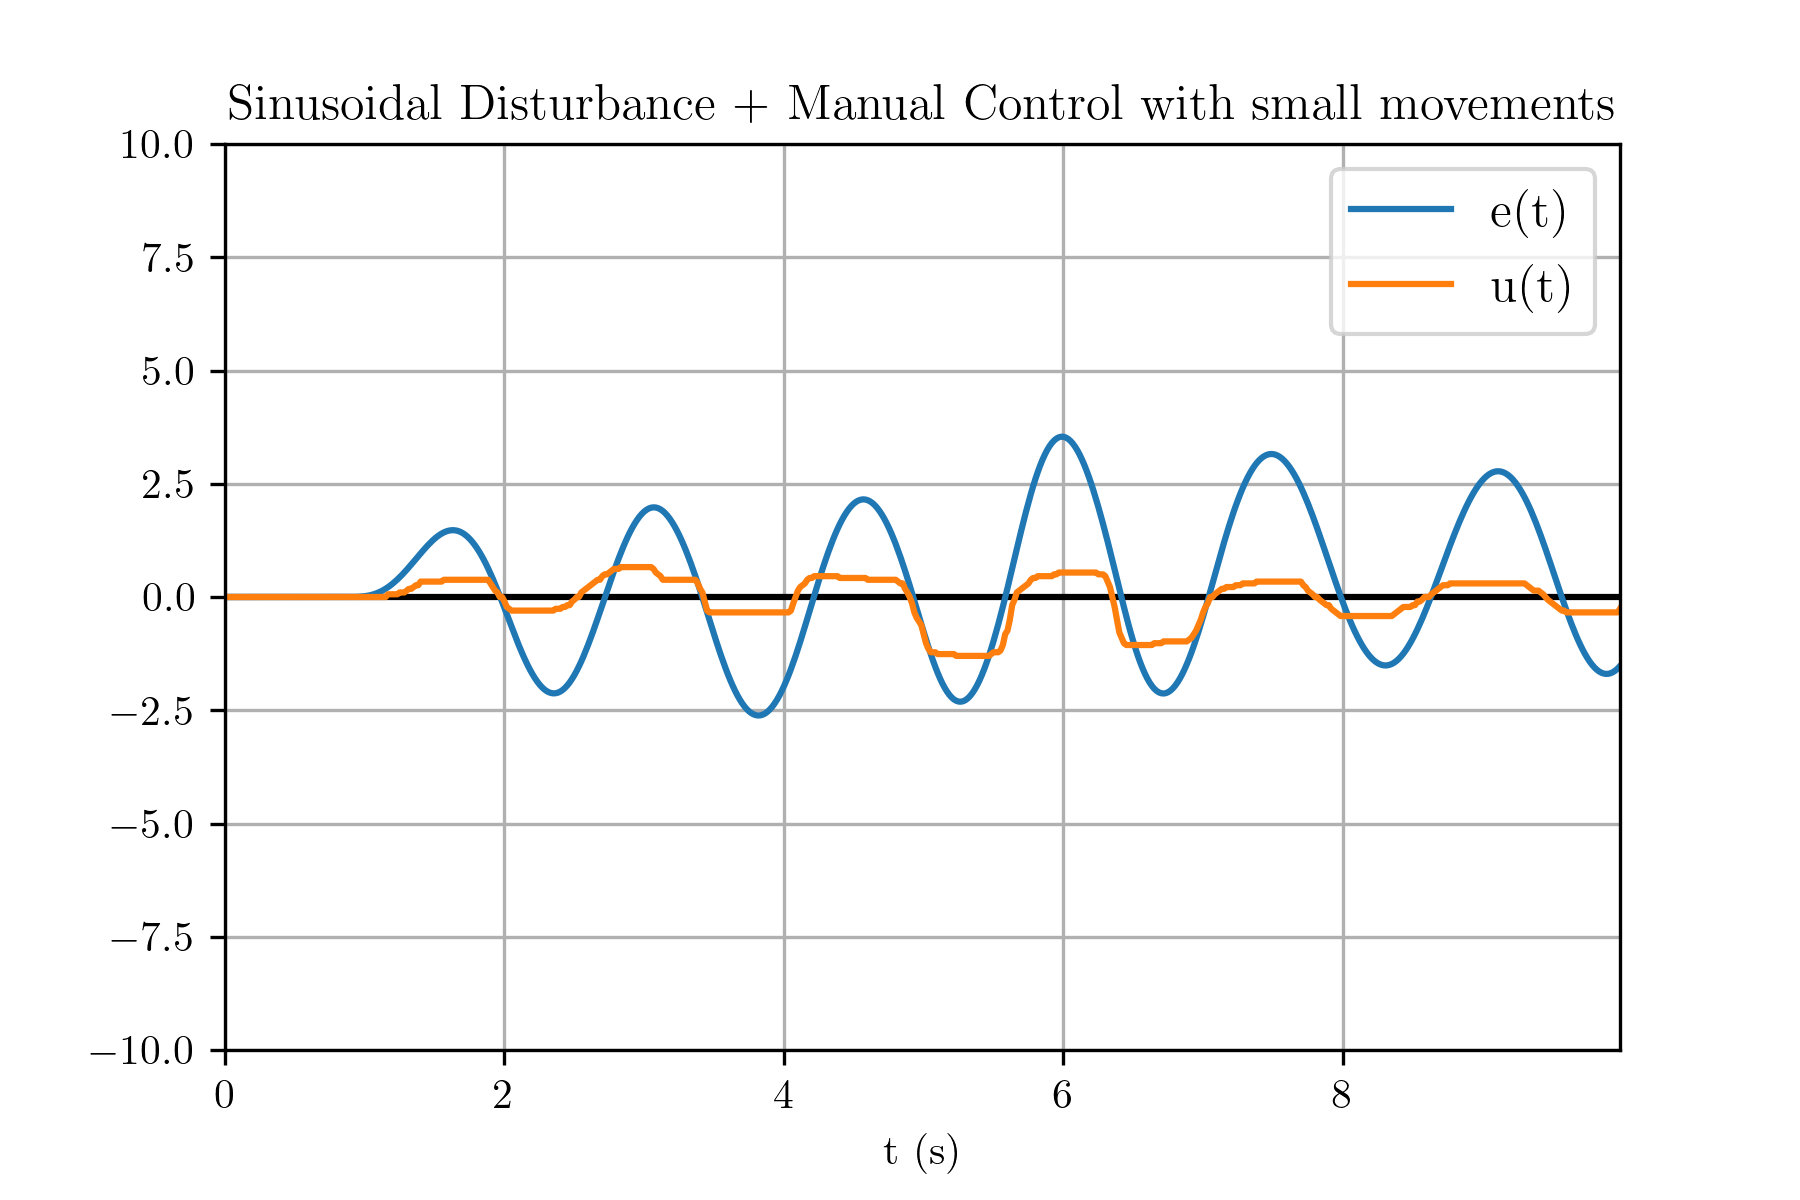
\includegraphics[width=1\textwidth]{figures/FIGURE_10.png}
        \caption{Small movement manual control input response with $0.66$ Hz sinusoidal disturbance.}
        \label{fig:figure10}
    \end{subfigure}
    \caption{F4E fighter jet responses}
\end{figure}

The response shown in Figure \ref{fig:figure8} with no controller, shows a smaller amplitude oscillatory response than with manual control.
This shows that this manual control is worse than no control for this case of disturbance and operating point of the aircraft.
The bode plot shown in Figure \ref{fig:figure9} shows that the point of resonance is very close to $\omega = 4.147$ rad/s or $0.66$ Hz.

From the red lines in figure \ref{fig:figure9}, the gain margin for the system was found to be 0.360.
This shows the maximum gain for which the system is stable and so stability could be achieved for small control inputs with the same controller delay of $0.250$s.

Figure \ref{fig:figure10} shows the response to small control movements. This shows significantly reduced error amplitudes than the previous manual input responses in figure \ref{fig:figure7}.
However, when compared to the no control response in figure \ref{fig:figure8}, the error amplitudes were comparable.
This shows that the pilot model controller is not effective at stabilising this case of disturbance and operating point of the aircraft.


\section{Unstable Aircraft}

\begin{equation}
    G_2(s) = \frac{2}{Ts-1}
\end{equation}

It can be seen that this aircrafts transfer function has a pole at $s=1/T$
An attempt to manually stabalise the system after a $0.1$ magnitude impulse disturbance with $T=0.7$ is shown below in Figure \ref{fig:figure11}.
At tested values of $T<0.7$, the system was more difficult to stabalise.

\begin{figure}[H]
    \centering
    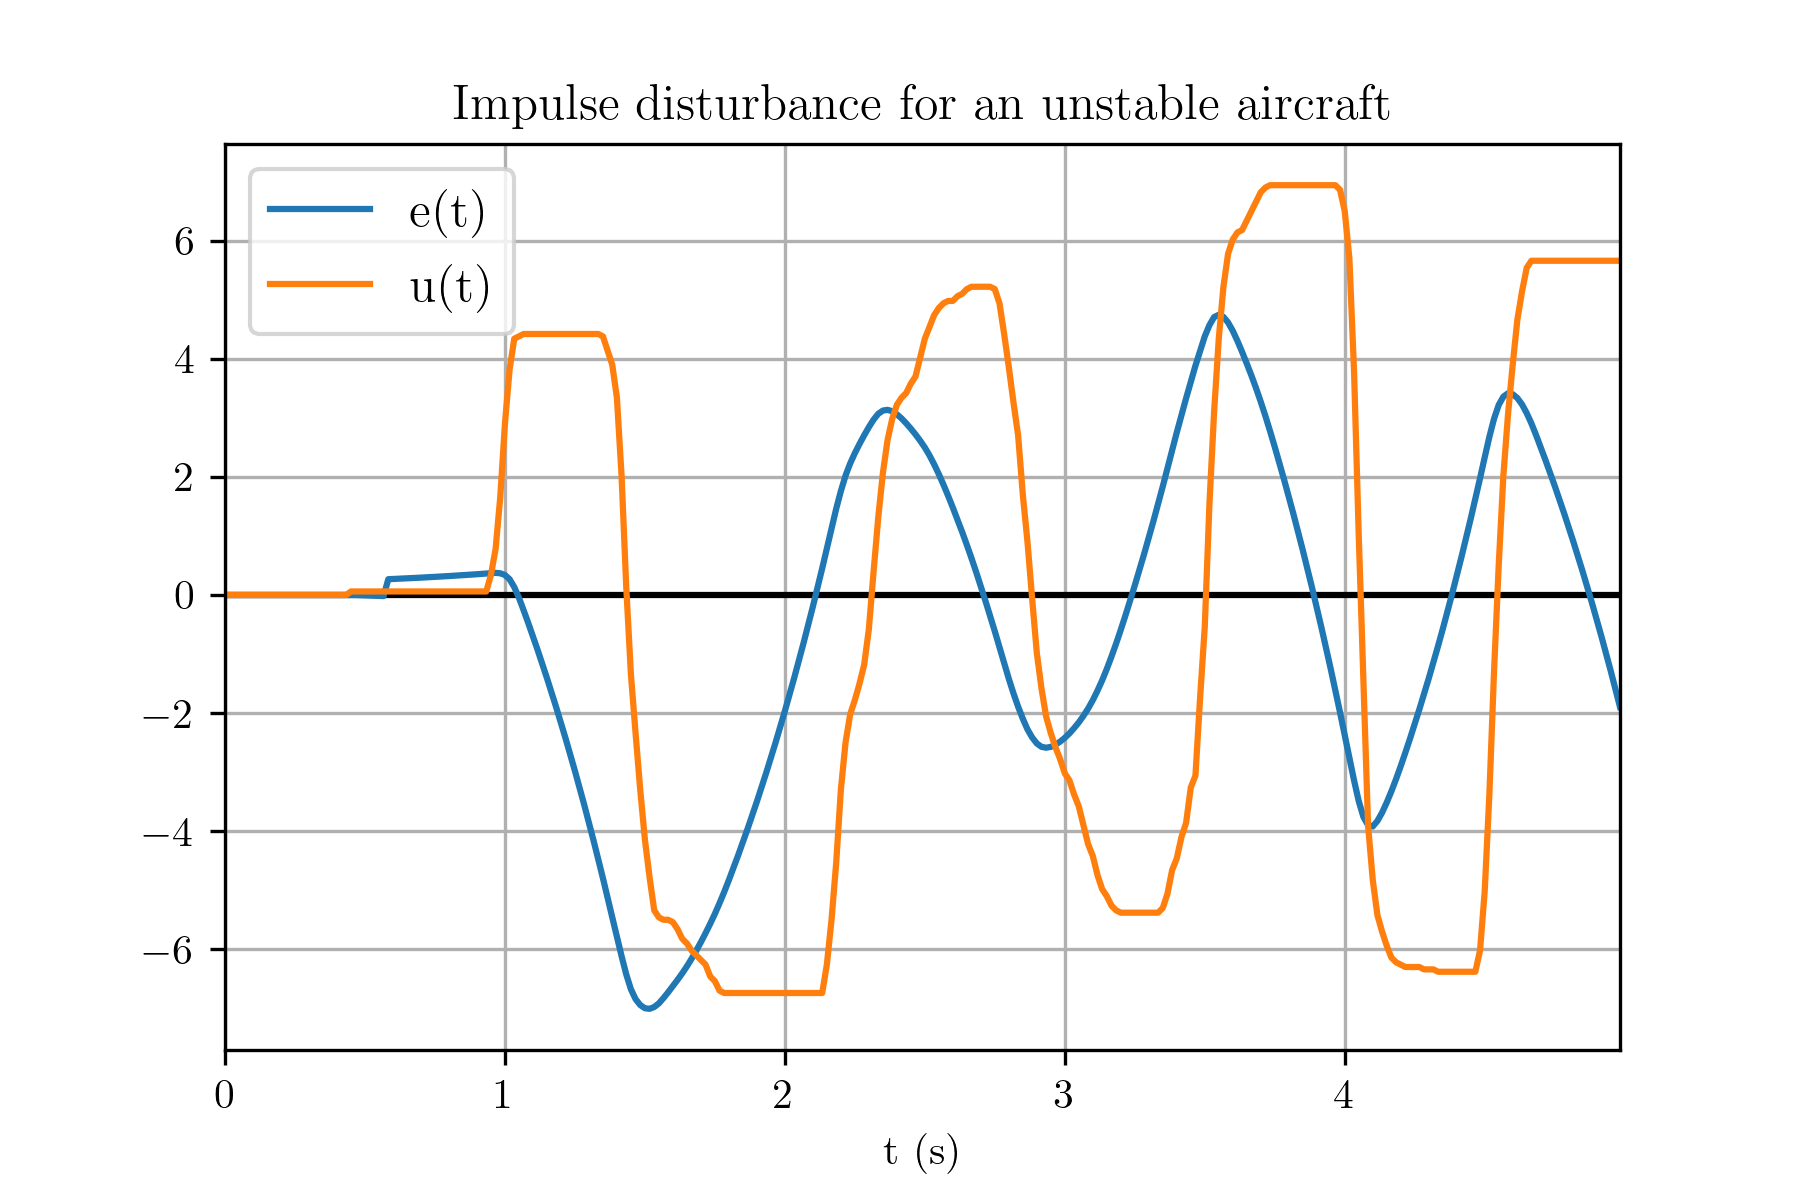
\includegraphics[width=0.8\textwidth]{figures/FIGURE_11.png}
    \caption{Manual control response to 0.1 magnitude impulse with $T=0.7$.}
    \label{fig:figure11}
\end{figure}


\begin{figure}[H]
    \centering
    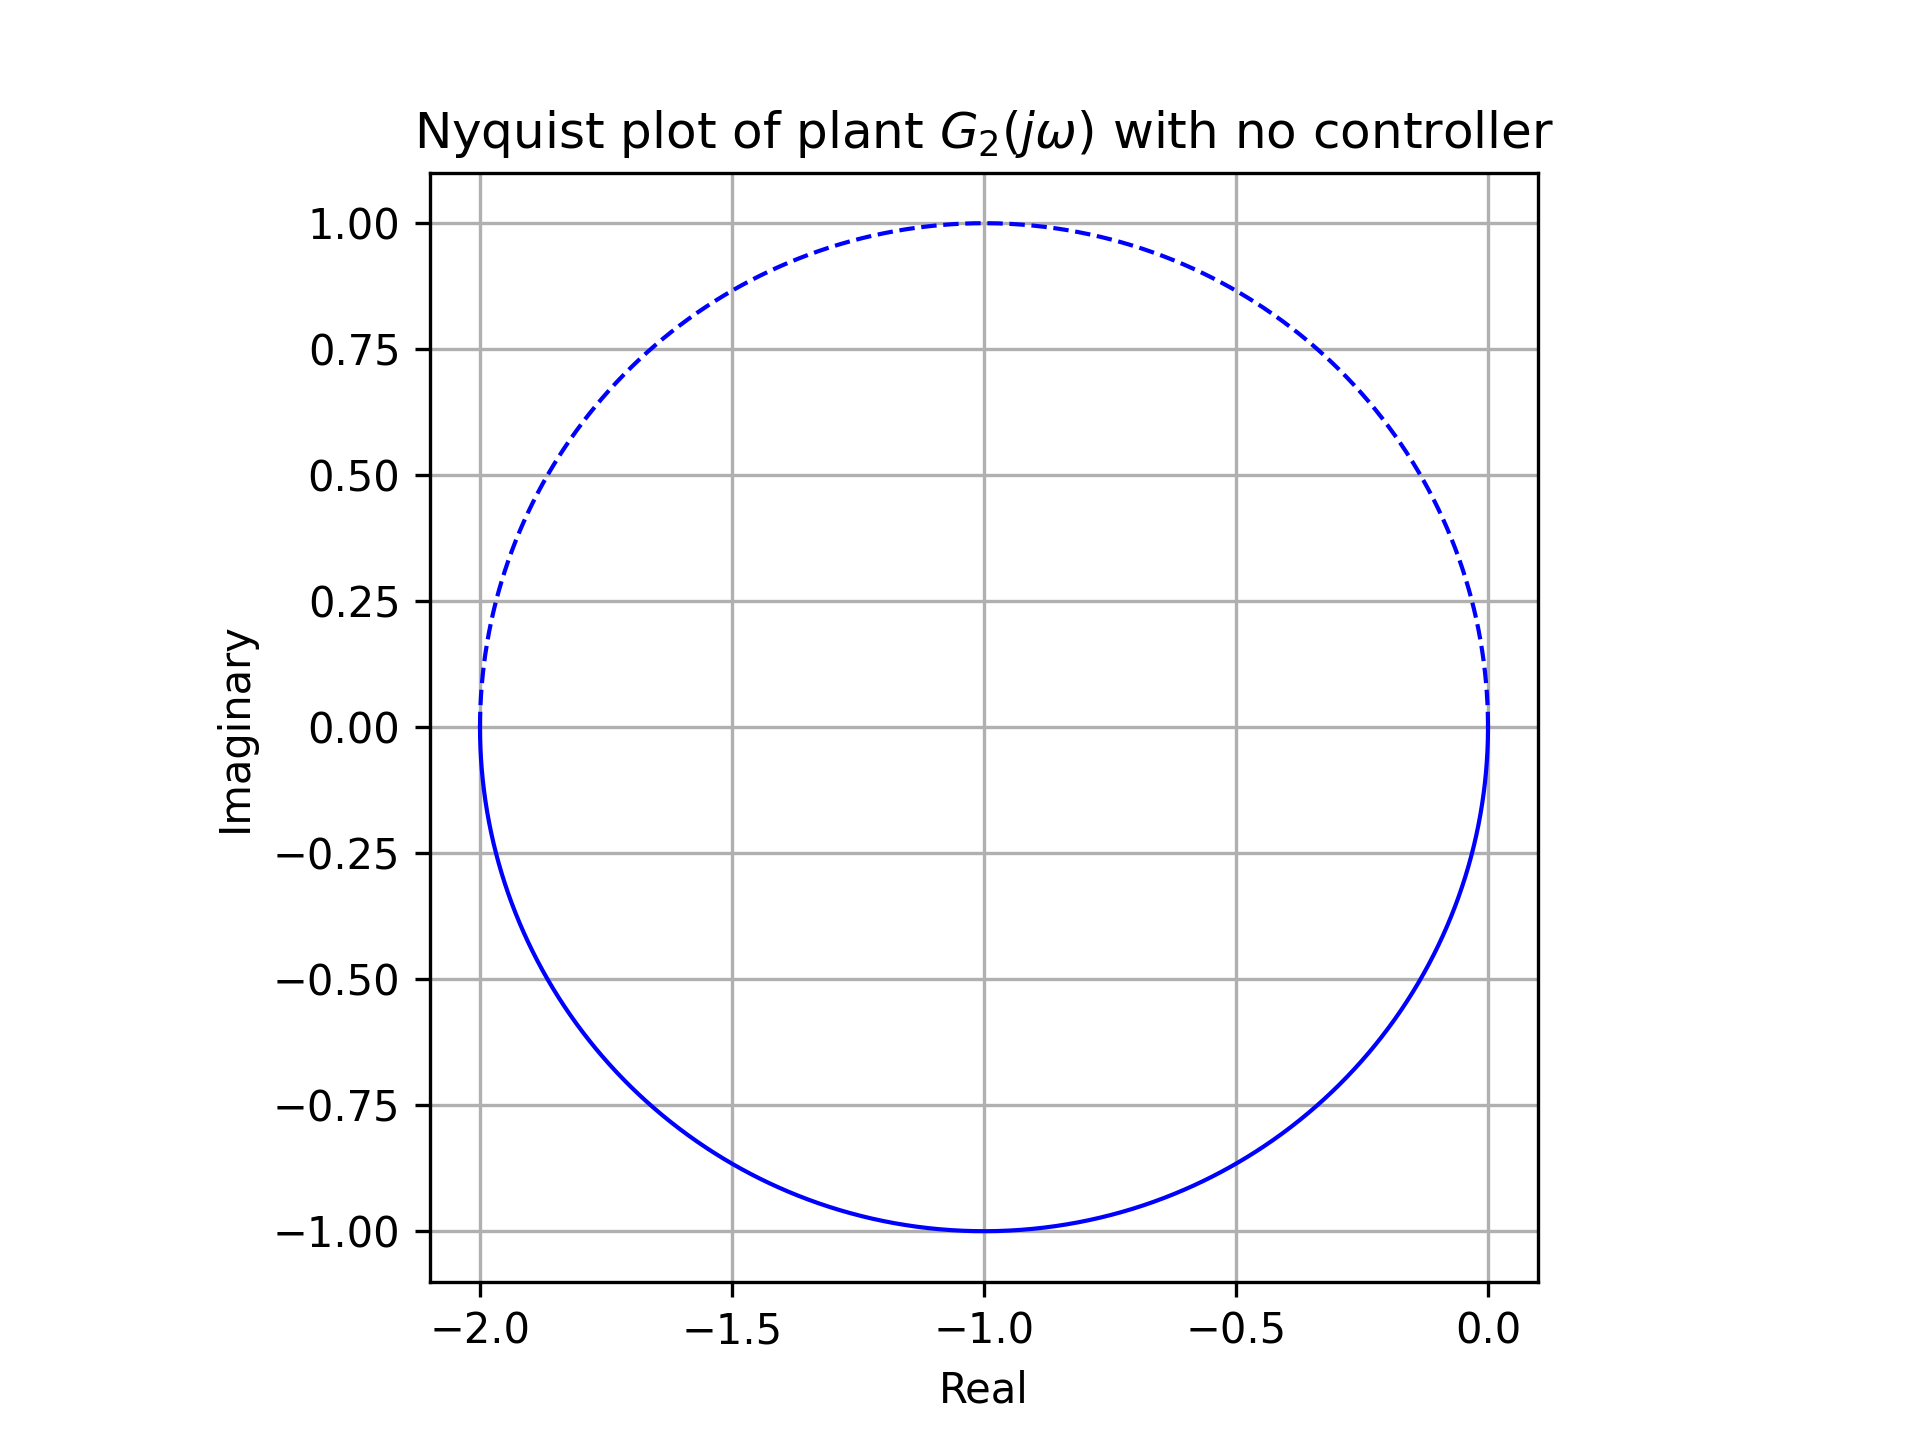
\includegraphics[width=0.8\textwidth]{figures/nyquist2.png}
    \caption{Nyquist plot of plant, $G_2(j\omega)$ with and without an additional delay, $D$.}
    \label{fig:nyquist2}
\end{figure}

The Nyquist plot in Figure \ref{fig:nyquist2} shows an anticlockwise encirclement of the -1 point and so the plant is unstable.
For the closed loop system to be stable, according to the Nyquist stability criterion, the number of anticlockwise encirclements of the -1 point must equal the number of unstable poles of the open loop system.
For this to be true in this case, $k>0.5$ such that the point -1 is always encircled once.

\section{Autopilot}

\begin{equation}
    G_3(s) = \frac{6.3s^2 + 4.3s + 0.28}{s^5 + 11.2s^4 + 19.6s^3 + 16.2s^2 + 0.91s + 0.27}
\end{equation}

\subsection{A Proportional controller}

The most simple controller is a proportional controller, which is given by the following equation:

\begin{equation}
    u(t) = K_p e(t)
\end{equation}

A large value of $K_p$ leads to smaller steady state error, but as we have seen, produces a more oscillatory response and can cause instability.
The value of $K_p$ of the autopilot was incrementally increased to find the critical gain $K_C$, for which the system appears marginally stable. This value should be close to the gain margin of the system.

\begin{figure}[H]
    \centering
    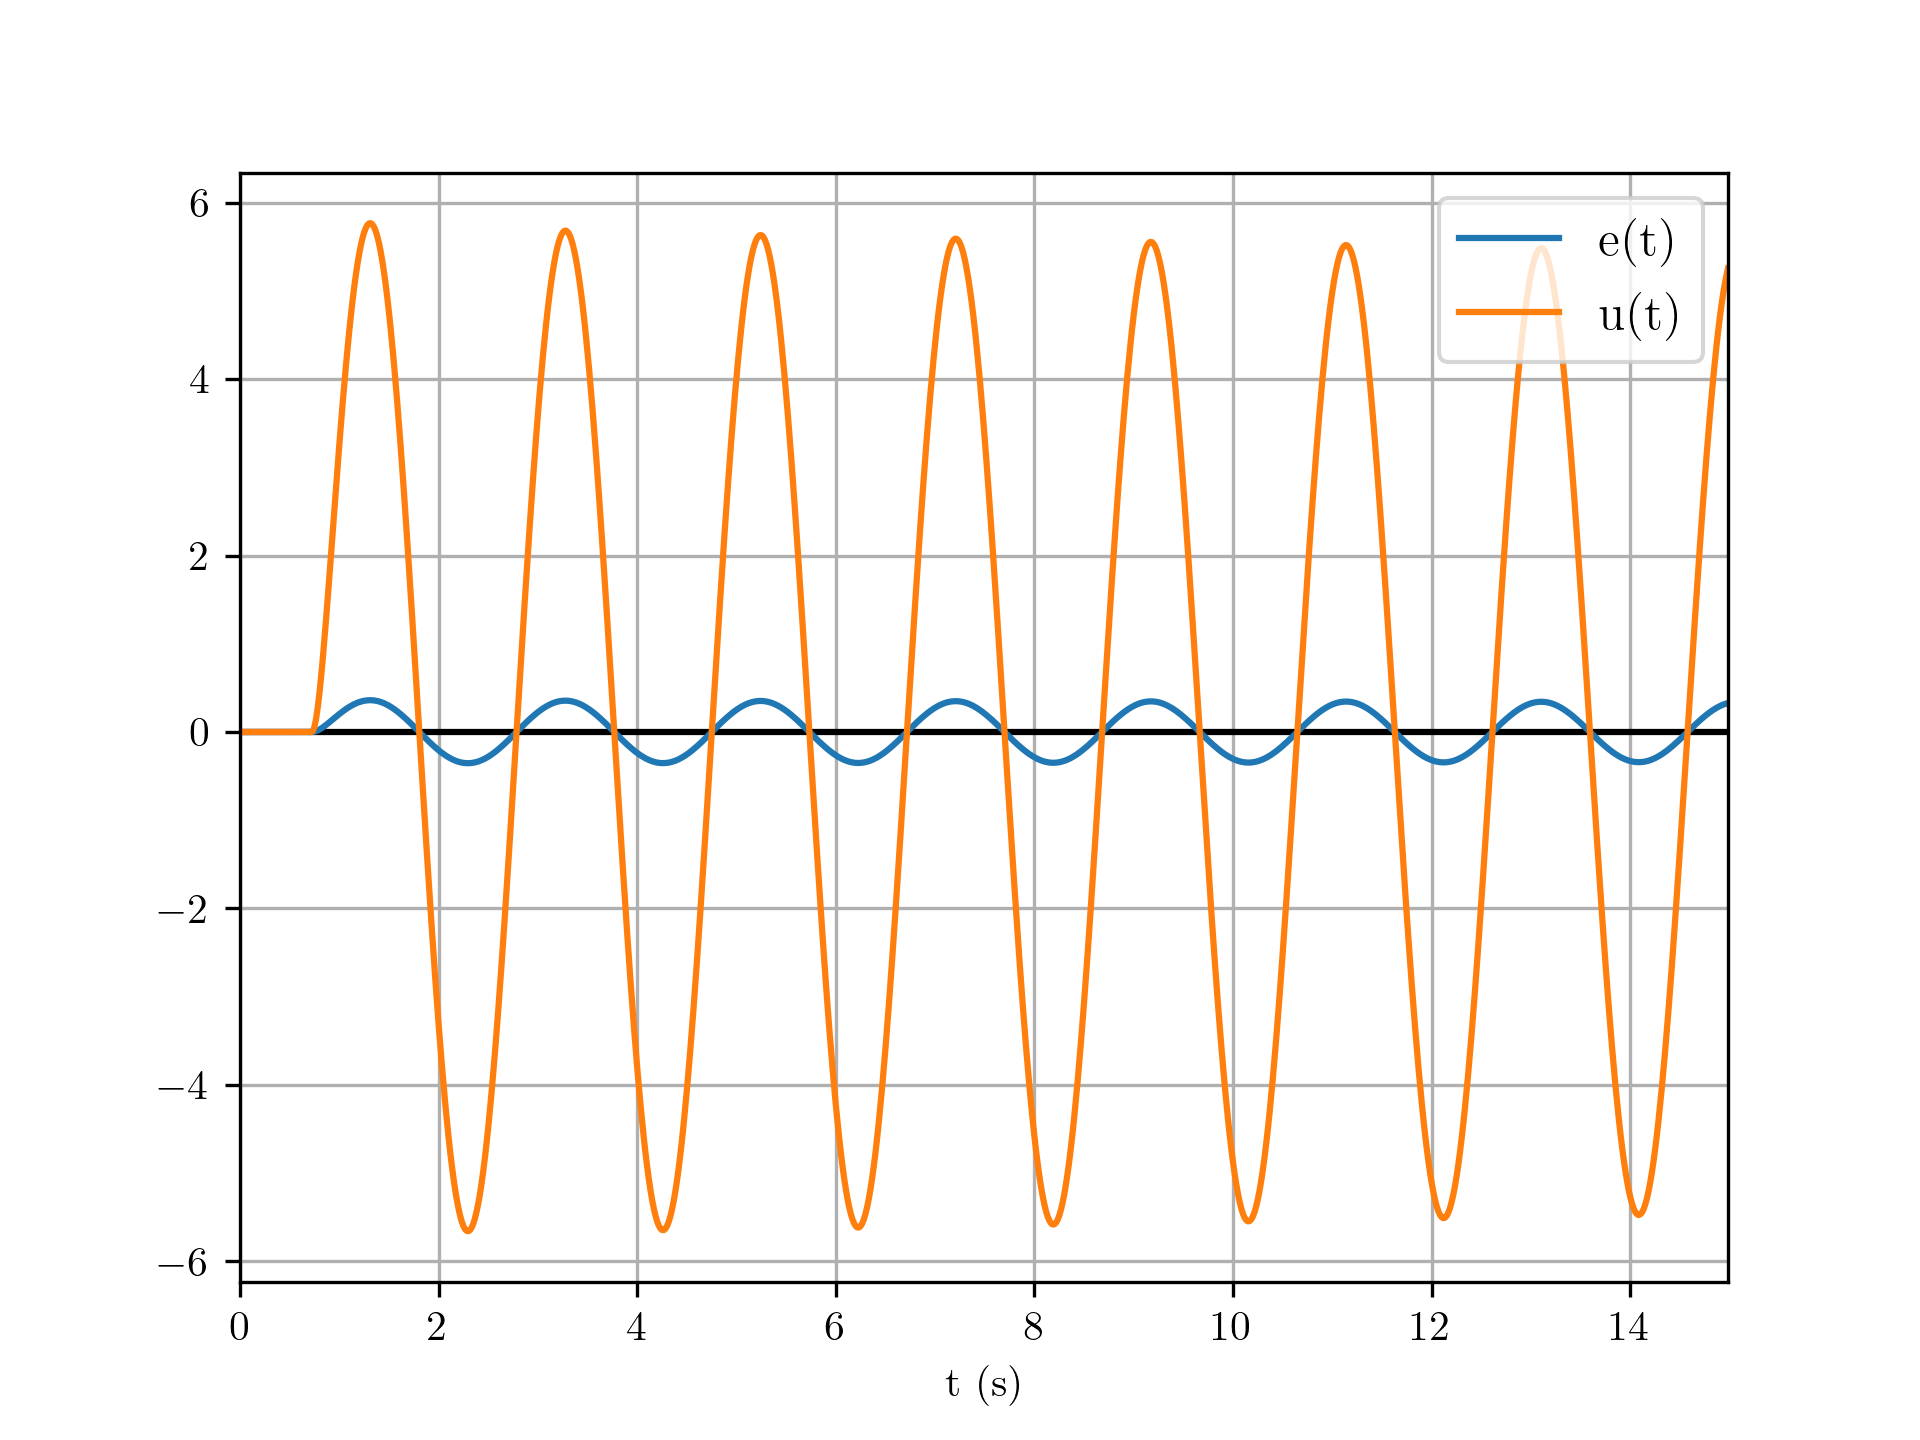
\includegraphics[width=0.8\textwidth]{figures/FIGURE_12.png}
    \caption{Proportional controller with value, $K_C$, response to impulse disturbance of weight $5$.}
    \label{fig:figure12}
\end{figure}

The value for critical gain was found to be $K_C = 16$
The corresponding critical period of oscillation was found to be $T_C = 1.967$ s.

\subsection{A PID Controller}

The PID controller consists of three terms, a proportional term, an integral term and a derivative term which can be seen below in both time and laplace domain.

\begin{equation}
    u(t) = K_p \left ( e(t) + \frac{1}{Ti}\int_{0}^{t}e(\tau)\mathrm{d}\tau + T_d\frac{\mathrm{d} e}{\mathrm{d} t} \right )
\end{equation}

\begin{equation}
    K(s) = K_p \left( 1 + \frac{1}{sT_i} + sT_d \right)
\end{equation}

The values of $K_p$, $T_i$ $T_d$ are set by the previous values of critical gain $K_C$ and $T_C$ according to the Zieger Nichols tuning method. This can be seen in the equations below.
\begin{equation}
    K_p=0.6K_c, \;\;\;\; T_i=0.5T_c, \;\;\;\; T_d = 0.125T_c
\end{equation}

These tuned values provide an effective controller for disturbance rejection.
Figures \ref{fig:figure125} and \ref{fig:figure13} show the response of the PID controller to a composite disturbance which is made up of both an impulse and a step disturbance.

\begin{figure}[H]
    \centering
    \begin{subfigure}[t]{0.48\textwidth}
        \centering
        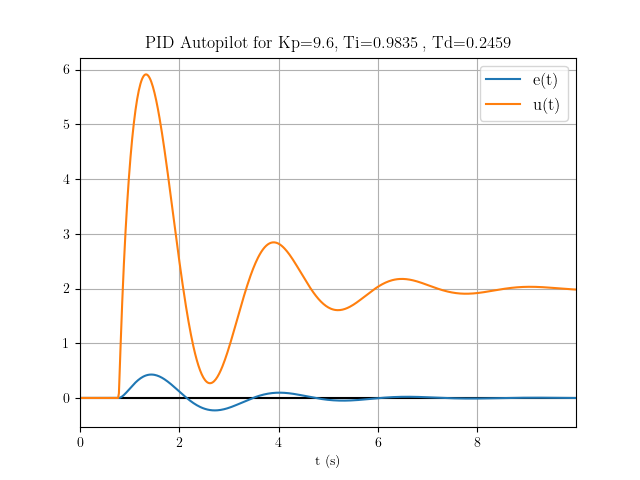
\includegraphics[width=1\textwidth]{figures/FIGURE_125.png}
        \caption{PID autopilot response to Composite disturbance.}
        \label{fig:figure125}
    \end{subfigure}
    ~
    \begin{subfigure}[t]{0.48\textwidth}
        \centering
        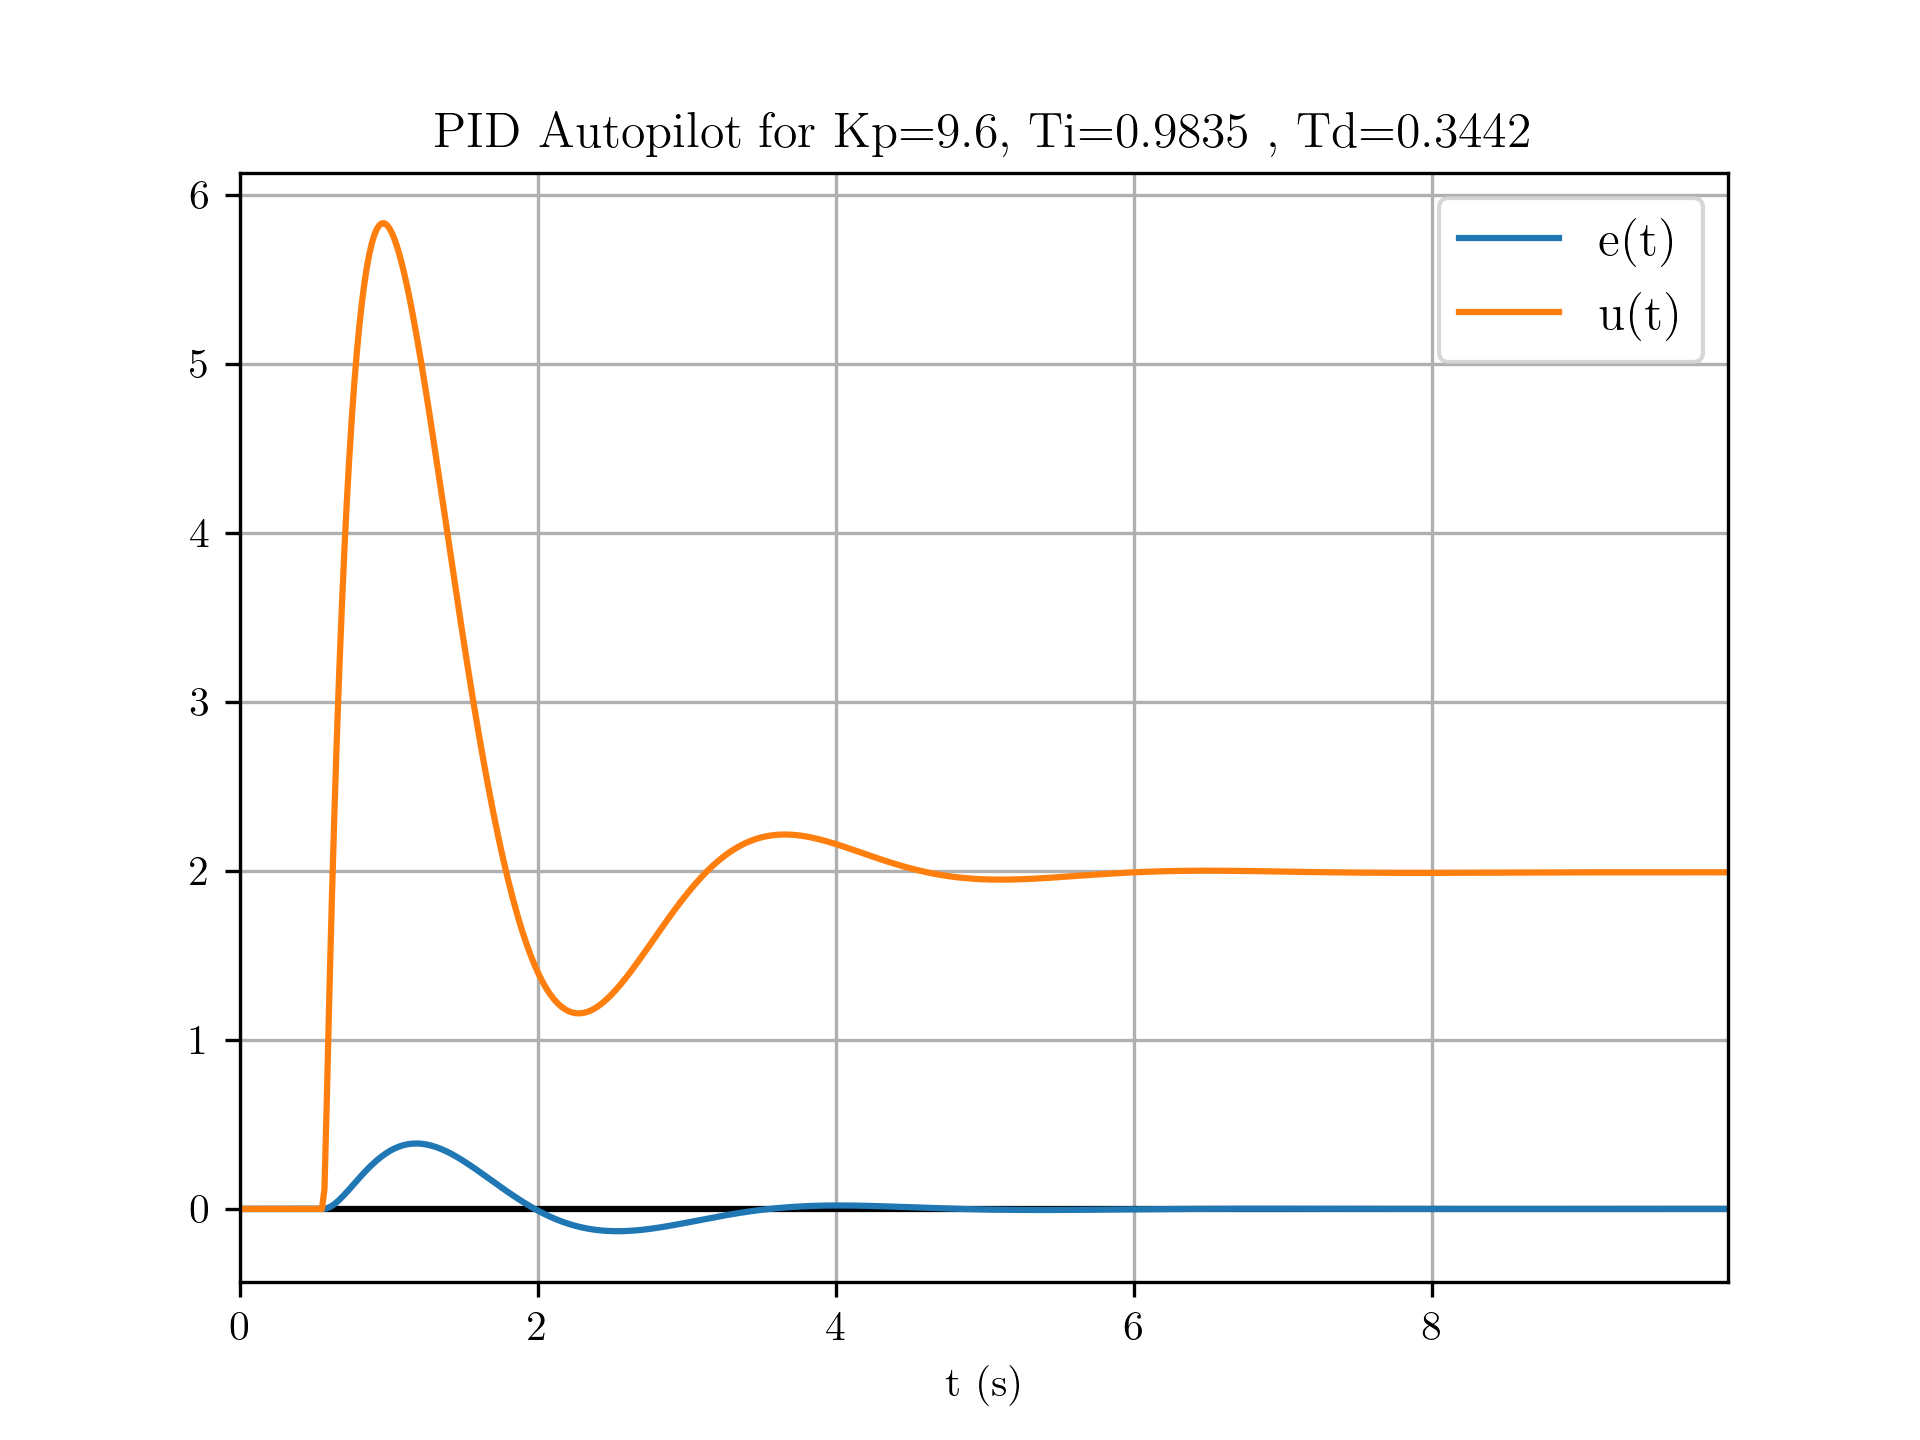
\includegraphics[width=1\textwidth]{figures/FIGURE_13.png}
        \caption{PID autopilot response with $40\%$ increase in $T_d$ to same Composite disturbance.}
        \label{fig:figure13}
    \end{subfigure}
    \caption{}
\end{figure}

From figures \ref{fig:figure125} and \ref{fig:figure13} it can be seen that increasing the derivative term $T_d$ by $40\%$ leads to faster disturbance rejection and a better autopilot system.

\subsection{Integrator wind up}

The integrator wind up problem occurs when the system is subject to a large disturbance, which causes the integrator to saturate.
This casues severe overshoot in order to reduce the integrator error.
A demonstation of this can be seen below in Figure \ref{fig:figure14}.
The easiest solution to this problem is to set a fixed bound on the integrator term, $Q$.

For a maximum steady state disturbance of $d$, the maximum integrator bound should be such that:

\begin{equation}
    d = \frac{K_p}{T_i}\int e(\tau)d\tau = \frac{K_p}{T_i}Q \implies Q = \frac{T_i}{K_p}d
\end{equation}

For a step disturbance of magnitude 2, the maximum integrator bound is $Q=0.1229$.

\begin{figure}[H]
    \centering
    \begin{subfigure}[t]{0.48\textwidth}
        \centering
        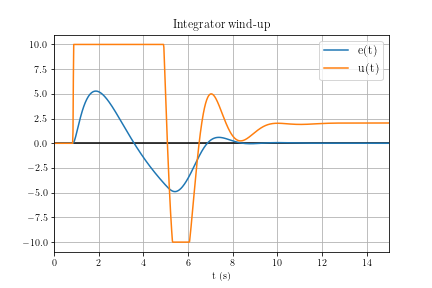
\includegraphics[width=1.0\textwidth]{figures/FIGURE_14.png}
        \caption{Autopilot response to composite disturbance.}
        \label{fig:figure14}
    \end{subfigure}
    ~
    \begin{subfigure}[t]{0.48\textwidth}
        \centering
        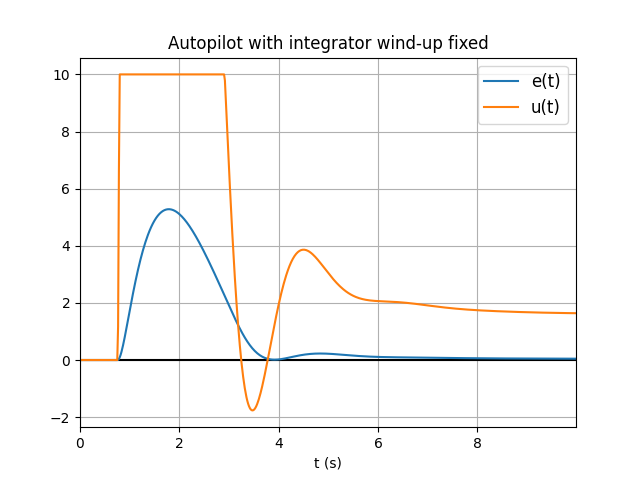
\includegraphics[width=1.0\textwidth]{figures/FIGURE_15.png}
        \caption{Autopilot with fixed integral wind up, $Q=0.1229$, response to same composite disturbance.}
        \label{fig:figure15}
    \end{subfigure}
    \caption{}
\end{figure}

Figure \ref{fig:figure14} shows the overshoot caused by the integrator wind up problem.
Figure \ref{fig:figure15} shows the response with a fixed integrator bound of $Q=0.1229$ with very little overshoot, and faster disturbance rejection.

\end{document}
